% Options for packages loaded elsewhere
\PassOptionsToPackage{unicode}{hyperref}
\PassOptionsToPackage{hyphens}{url}
%
\documentclass[
]{article}
\usepackage{amsmath,amssymb}
\usepackage{lmodern}
\usepackage{iftex}
\ifPDFTeX
  \usepackage[T1]{fontenc}
  \usepackage[utf8]{inputenc}
  \usepackage{textcomp} % provide euro and other symbols
\else % if luatex or xetex
  \usepackage{unicode-math}
  \defaultfontfeatures{Scale=MatchLowercase}
  \defaultfontfeatures[\rmfamily]{Ligatures=TeX,Scale=1}
\fi
% Use upquote if available, for straight quotes in verbatim environments
\IfFileExists{upquote.sty}{\usepackage{upquote}}{}
\IfFileExists{microtype.sty}{% use microtype if available
  \usepackage[]{microtype}
  \UseMicrotypeSet[protrusion]{basicmath} % disable protrusion for tt fonts
}{}
\makeatletter
\@ifundefined{KOMAClassName}{% if non-KOMA class
  \IfFileExists{parskip.sty}{%
    \usepackage{parskip}
  }{% else
    \setlength{\parindent}{0pt}
    \setlength{\parskip}{6pt plus 2pt minus 1pt}}
}{% if KOMA class
  \KOMAoptions{parskip=half}}
\makeatother
\usepackage{xcolor}
\IfFileExists{xurl.sty}{\usepackage{xurl}}{} % add URL line breaks if available
\IfFileExists{bookmark.sty}{\usepackage{bookmark}}{\usepackage{hyperref}}
\hypersetup{
  pdftitle={Multivariate State Space Models for Neuropsychological Cognitive Scores},
  pdfauthor={Zach Baucom, BS, zhbaucom@bu.edu; Yorghos Tripodis, PhD, yorghos@bu.edu; Michael Alosco, PhD, malsoco@bu.edu; Evan Johnson, PhD, wej@bu.edu},
  hidelinks,
  pdfcreator={LaTeX via pandoc}}
\urlstyle{same} % disable monospaced font for URLs
\usepackage[margin=1in]{geometry}
\usepackage{longtable,booktabs,array}
\usepackage{calc} % for calculating minipage widths
% Correct order of tables after \paragraph or \subparagraph
\usepackage{etoolbox}
\makeatletter
\patchcmd\longtable{\par}{\if@noskipsec\mbox{}\fi\par}{}{}
\makeatother
% Allow footnotes in longtable head/foot
\IfFileExists{footnotehyper.sty}{\usepackage{footnotehyper}}{\usepackage{footnote}}
\makesavenoteenv{longtable}
\usepackage{graphicx}
\makeatletter
\def\maxwidth{\ifdim\Gin@nat@width>\linewidth\linewidth\else\Gin@nat@width\fi}
\def\maxheight{\ifdim\Gin@nat@height>\textheight\textheight\else\Gin@nat@height\fi}
\makeatother
% Scale images if necessary, so that they will not overflow the page
% margins by default, and it is still possible to overwrite the defaults
% using explicit options in \includegraphics[width, height, ...]{}
\setkeys{Gin}{width=\maxwidth,height=\maxheight,keepaspectratio}
% Set default figure placement to htbp
\makeatletter
\def\fps@figure{htbp}
\makeatother
\setlength{\emergencystretch}{3em} % prevent overfull lines
\providecommand{\tightlist}{%
  \setlength{\itemsep}{0pt}\setlength{\parskip}{0pt}}
\setcounter{secnumdepth}{5}
\newlength{\cslhangindent}
\setlength{\cslhangindent}{1.5em}
\newlength{\csllabelwidth}
\setlength{\csllabelwidth}{3em}
\newlength{\cslentryspacingunit} % times entry-spacing
\setlength{\cslentryspacingunit}{\parskip}
\newenvironment{CSLReferences}[2] % #1 hanging-ident, #2 entry spacing
 {% don't indent paragraphs
  \setlength{\parindent}{0pt}
  % turn on hanging indent if param 1 is 1
  \ifodd #1
  \let\oldpar\par
  \def\par{\hangindent=\cslhangindent\oldpar}
  \fi
  % set entry spacing
  \setlength{\parskip}{#2\cslentryspacingunit}
 }%
 {}
\usepackage{calc}
\newcommand{\CSLBlock}[1]{#1\hfill\break}
\newcommand{\CSLLeftMargin}[1]{\parbox[t]{\csllabelwidth}{#1}}
\newcommand{\CSLRightInline}[1]{\parbox[t]{\linewidth - \csllabelwidth}{#1}\break}
\newcommand{\CSLIndent}[1]{\hspace{\cslhangindent}#1}
\usepackage{booktabs}
\usepackage{longtable}
\usepackage{array}
\usepackage{multirow}
\usepackage{wrapfig}
\usepackage{float}
\usepackage{colortbl}
\usepackage{pdflscape}
\usepackage{tabu}
\usepackage{threeparttable}
\usepackage{threeparttablex}
\usepackage[normalem]{ulem}
\usepackage{makecell}
\usepackage{xcolor}
\usepackage{amsmath}
\usepackage{algorithm,algorithmic}
\addtolength{\oddsidemargin}{-.5in}%
\addtolength{\evensidemargin}{-.5in}%
\addtolength{\textwidth}{1in}%
\addtolength{\textheight}{-.3in}%
\addtolength{\topmargin}{-.8in}%
\usepackage{float}
\floatplacement{figure}{H}
\usepackage{booktabs}
\usepackage{longtable}
\usepackage{array}
\usepackage{multirow}
\usepackage{wrapfig}
\usepackage{float}
\usepackage{colortbl}
\usepackage{pdflscape}
\usepackage{tabu}
\usepackage{threeparttable}
\usepackage{threeparttablex}
\usepackage[normalem]{ulem}
\usepackage{makecell}
\usepackage{xcolor}
\ifLuaTeX
  \usepackage{selnolig}  % disable illegal ligatures
\fi

\title{Multivariate State Space Models for Neuropsychological Cognitive Scores}
\author{Zach Baucom, BS, \href{mailto:zhbaucom@bu.edu}{\nolinkurl{zhbaucom@bu.edu}} \and Yorghos Tripodis, PhD, \href{mailto:yorghos@bu.edu}{\nolinkurl{yorghos@bu.edu}} \and Michael Alosco, PhD, \href{mailto:malsoco@bu.edu}{\nolinkurl{malsoco@bu.edu}} \and Evan Johnson, PhD, \href{mailto:wej@bu.edu}{\nolinkurl{wej@bu.edu}}}
\date{}

\begin{document}
\maketitle

{
\setcounter{tocdepth}{2}
\tableofcontents
}
\newpage{}

\hypertarget{introduction}{%
\section{Introduction}\label{introduction}}

Alzheimer's Disease (AD) is a neurodegenerative disease that affects tens of millions of people world-wide and the prevalence is expected to increase with the aging of the baby boomer population. AD is related to a protein build-up in the brain, leading to brain matter deterioration. Brain deterioration often presents itself outwardly in the form of a decreased ability to perform simple tasks and provide for oneself. The impact of AD is costly. The ({``2022 Alzheimer's Disease Facts and Figures''} 2022) estimates that \$271 billion in unpaid care was accumulated for those living with AD in 2021. This does not take into account the emotional toll of caring for a loved one suffering from AD. Although testing for biomarkers or providing brain scans can be effective in diagnosing AD, understanding the overall cognition process for those suffering with Alzheimer's Disease (AD) has been an emerging line of statistical research. Defining this process can lead to early diagnosis and the implementation of possible interventions to create positive impacts for those suffering with AD and their caretakers. Cognition, however, is complex, multifaceted, and is measured indirectly.

Much research has been undertaken to describe the cognitive process of AD. Large organizations, like the National Alzheimer's Coordinating Center (NACC), offer a battery of repeated neuropsychological tests in order to best estimate cognition as a whole as well as across different cognitive domains over time. Each neuropsychological test has known properties and is related by construction to one or several cognitive domains. The NACC battery include tests related to memory (Logical Memory Immediate and Delayed), attention and psychomotor speed (WAIS, Trailmaking A, Digit Backward and Forward), executive function (Trailmaking B), and language (Boston Naming Test, Animals and Vegetables). This is vital as different domains of cognition are not homogeneous in their timing or rate of decline through the AD process {[}{]}. These tests implicitly include a measurement error which would decrease variability and potentially lead to conflicting conclusions. With the obvious shortcomings in modeling a single neuropsychological test, a number of studies rely on multivariate methods on a battery of tests to describe the domains of cognition. The cross-sectional study (Chapman et al. 2010) uses dimensionality reduction techniques to estimate prominent latent factors of AD at a single measurement time. The study (HAYDEN et al. 2011) seeks to improve on this study by separately computing factors at two different moments in time for those impaired and unimpaired.

A cross-sectional study aims to estimate the latent factors of cognition at a single moment in time, rather than taking into account a subject's cognition process through time. This design will be insufficient in describing the dynamic AD progression. In addition, a cross-sectional study could lead to an increased amount of variability as participants may not be in the same stage of AD progression. Although having multiple measurement can help, controlling for variation in cognitive trajectory that may be due to age, gender, sex, education, genetics, or other possible causes over time is needed as latent factors could be due to cohort differences.

In order to gain more accurate insight into latent factors of cognitive decline, we propose the use of a Bayesian estimated Multivariate Local Linear Trend Model (MLLT). The MLLT is an extension of the Local Linear Trend model (LLT) described in {[}Paper1{]} which was shown to accurately estimate effects on cognitive trajectory by allowing for a latent underlying cognition process. The proposed MLLT differs from the LLT in that it allows for the estimation of within subject correlation in the latent cognitive processes and the observation error for each respective outcome. The correlation of the latent cognitive process provides insight into the constructs of cognition and how they correlate through time. This model stands out as it estimates inter-relatedness of cognitive processes for each test while also accounting for unique cohort characteristic. The proposed MLLT can be neatly modeled using a similar Bayesian Gibb's sampling process as was shown in {[}paper1{]}.

To test the validity of the MLLT, we start by comparing the MLLT methods to independent LLT estimation when controlling the underlying data generation process. By controlling the underlying data generation process, we are able to verify the MLLT effectiveness against the chosen true data generation parameters. This simulation study not only verifies the effectiveness of the MLLTs ability to accurately estimate cross-test correlation at varying levels, but also illustrates deficiencies of independently estimating different cognition scores.

The MLLT model is then compared to independent LLTs when estimating a simulated linear effect on a battery of real tests offered by the NACC. When adding a linear effect, we know the parameter we want to estimate correctly, but we do not know the underlying cognition process. Accurate estimation of the added linear effect is indicative that the proposed model fits the data well and estimating the correlation in the underlying cognition processes is appropriate. In this real data simulation we show that the MLLT is just as accurate as the LLT at estimating linear effects of interest, but also has the added ability to offer more accurate insights into the cognition process over time.

After verifying the MLLT's added benefits, we fit the proposed model to data provided by the NACC. From our model, we show compelling insight into how underlying cognition processes vary for those with and without dementia. This analysis provides a clearer picture of cognitive decline as it pertains to AD. The multivariate local linear trend model is shown to fit the nueropsychological data provided by the NACC very well. The ability to control for cohort characteristics while estimating underlying congitive constructs in a longitudinal manner make this model dynamic and accurate.

\hypertarget{methods}{%
\section{Methods}\label{methods}}

\hypertarget{model-of-interest-and-data}{%
\subsection{Model of Interest and Data}\label{model-of-interest-and-data}}

\hypertarget{MOI}{%
\subsubsection{Model of Interest}\label{MOI}}

After controlling for the linear effects of dementia status (1 = diagnosed with MCI or dementia, 0 = otherwise), sex (1 = female, 0 = male), race (1 = white, 0 = other), age (mean centered), education (mean centered), and APOE e4 allele status (1 = has at least 1 APOE e4 allele, 0 = otherwise), we wish to compare latent cognition processes between those who have transitioned to MCI or dementia during follow-up (transitioners) and those who have not (non-transitioners). Previous research suggests that the effect of APOE e4 status differs between males and females, therefore an interaction between e4 status and sex is included in the model. To measure the linear effect of the dependent variables on the cognition tests trajectory, all dependent variables are put into the model as an interaction with time. In the group that have transitioned to MCI or dementia, we include a linear spline for when the participant transitions from cognitively normal to MCI or dementia.

\hypertarget{DAT}{%
\subsubsection{Data}\label{DAT}}

Data collected by the National Alzheimer's Coordinating Center (NACC) Uniform Data Set Version 2.0 (UDS, September 2014) was used to test the proposed MLLT model validity. The data analysis utilized two different groups in the NACC. Criteria for entry into the the first group requires Alzheimer's disease participants to have transitioned from cognitively normal to mild cognitive impairment (MCI) or Dementia during the NACC follow-up period. The second group are those who remained cognitively normal throughout the follow-up period. For the multivariate modeling of different cognition domains, we used the following neuropsychological outcomes: logic memory, memory units, digit forward, digit backward, trails A, trails B, WAIS, boston naming, and animals naming. Predictors of interest include: time, race white, sex, apoe e4 status, education, time of transition from cognitively normal to mild cognitive impairment (MCI) or dementia, and age. Inclusion into the analysis requires non-missingness for covariates and cognitive outcome at a given time point, as well as each participant needing 1 or more complete observation.

That are several cohort demographic differences in those who transitioned to MCI or dementia and those with no dementia diagnosis. As expected, transitioners are typically older at enrollment (78.45 years vs.~70.83 years), have more return visits into their older age (5.13 visits vs.~4.46 visits), and have higher rates of having an APOE e4 allele (38.26\% vs.~26.99\%). To assure latent cognition process correlations between dementia transitioners and non-dementia transitioners only differ due to dementia status, we conduct a sensitivity analysis with a more homogenous comparison group. To do this, we carry out 1-to-1 propensity matching with a caliper of 0.1 using all described linear predictors. Of the 737 transitioners, 734 matched to non-transitioners. In the transitioner and non-transitioner groups there is more similarity in enrollment age (78.40 years vs 78.44), return visits (5.13 visits vs.~5.25 visits), and e4 allele status (38.15\% vs.~38.15\%).

\begin{table}

\caption{\label{tab:unnamed-chunk-12}Demographic description for matched and unmatched datasets.}
\centering
\begin{tabular}[t]{lllll}
\toprule
\multicolumn{1}{c}{ } & \multicolumn{2}{c}{Non-Matched} & \multicolumn{2}{c}{Matched} \\
\cmidrule(l{3pt}r{3pt}){2-3} \cmidrule(l{3pt}r{3pt}){4-5}
  & Dementia & Non-Dementia & Dementia & Non-Dementia\\
\midrule
N participants & 737 & 6136 & 734 & 734\\
Return visits & 5.13 (2.06) & 4.46 (2.24) & 5.13 (2.05) & 5.25 (2.33)\\
APOE e4 allele & 38.26\% & 26.99\% & 38.15\% & 35.15\%\\
Sex (female) & 62.69\% & 67.42\% & 62.53\% & 62.13\%\\
Race (white) & 87.65\% & 83.34\% & 87.6\% & 87.87\%\\
\addlinespace
Age & 78.45 (8.25) & 70.83 (10.18) & 78.4 (8.23) & 78.44 (8.45)\\
Education yrs & 16.14 (8.11) & 16.13 (5.95) & 16.02 (7.53) & 15.83 (4.28)\\
Follow-up trs & 5.02 (2.17) & 4.18 (2.48) & 5.01 (2.16) & 5.14 (2.5)\\
Time of decline
(tears since baseline) & 3.54 (2.11) & - & 3.53 (2.1) & -\\
\bottomrule
\end{tabular}
\end{table}

\hypertarget{proposed-multivariate-model}{%
\subsection{Proposed Multivariate Model}\label{proposed-multivariate-model}}

Fitting a multivariate LLT allows for the measurement in similarity of underlying constructs for different cognitive tests and compare the effect of some variable across different tests e.g.~does APOE have a significantly different effect on cognitive trajectory for the Trails A and Trails B tests? Let \(y_{ijk}\) represent the outcome of cognitive test \(k\in \{1, 2, 3, ..., K\}\) at time \(j\in \{1, 2, 3, ..., J\}\) for subject \(i \in \{1, 2, 3, ..., N\}\). The model can then be formulated as,

\begin{equation*}
\begin{aligned}
\begin{bmatrix}
y_{ij1}\\
y_{ij2}\\
\vdots\\
y_{ijK}
\end{bmatrix}
&= \begin{bmatrix}
\alpha_{ij1}\\
\alpha_{ij2}\\
\vdots\\
\alpha_{ijK}
\end{bmatrix}
+ 
\begin{bmatrix}
\boldsymbol{x_{ij}\beta_1}\\
\boldsymbol{x_{ij}\beta_2}\\
\vdots\\
\boldsymbol{x_{ij}\beta_K} 
\end{bmatrix} +
\begin{bmatrix}
\varepsilon_{ij1}\\
\varepsilon_{ij2}\\
\vdots\\
\varepsilon_{ijK}
\end{bmatrix},  
\begin{bmatrix}
\varepsilon_{ij1}\\
\varepsilon_{ij2}\\
\vdots\\
\varepsilon_{ijK}
\end{bmatrix} 
\sim N(0, \Sigma_\varepsilon
)\\
\begin{bmatrix}
\alpha_{ij1}\\
\alpha_{ij2}\\
\vdots\\
\alpha_{ijK}
\end{bmatrix} & = 
\begin{bmatrix}
\alpha_{i(j-1)1}\\
\alpha_{i(j-1)2}\\
\vdots\\
\alpha_{i(j-1)K}
\end{bmatrix} +
\begin{bmatrix}
\eta_{ij1}\\
\eta_{ij2}\\
\vdots\\
\eta_{ijK}
\end{bmatrix}, 
\begin{bmatrix}
\eta_{ij1}\\
\eta_{ij2}\\
\vdots\\
\eta_{ijK}
\end{bmatrix} \sim N(0, \delta_{ij}\Sigma_\eta)
\end{aligned}
\end{equation*}

In this model representation, \(\Sigma_\varepsilon \in R^{KxK}\) and \(\Sigma_\eta \in R^{KxK}\). Utilizing \(\Sigma_\varepsilon\) and \(\Sigma_\eta\) allows for estimation of correlation between cognitive tests. However, allowing for non-zero elements in the non-diagonal adds a possibly large number of parameters to estimate. We propose the use of three different models,

Model O: Correlation is in Measurement eq.

\begin{equation*}
\begin{aligned}
\Sigma_\varepsilon =
\begin{bmatrix}
\sigma^{2(1)}_\varepsilon & \sigma^{2(1,2)}_\varepsilon & \cdots & \sigma^{2(1, K)}_\varepsilon\\
\sigma^{2(1,2)}_\varepsilon & \sigma^{2(2)}_\varepsilon\\
\vdots & & \ddots\\
\sigma^{2(1, K)}_\varepsilon & & &\sigma^{2(K)}_\varepsilon
\end{bmatrix},
\Sigma_\eta = 
\begin{bmatrix}
\sigma^{2(1)}_\eta & 0 & \cdots & 0\\
0 & \sigma^{2(2)}_\eta\\
\vdots & & \ddots\\
0 & & &\sigma^{2(K)}_\eta
\end{bmatrix}
\end{aligned}
\end{equation*}

Model S: Correlation is in State eq.

\begin{equation*}
\begin{aligned}
\Sigma_\varepsilon = 
\begin{bmatrix}
\sigma^{2(1)}_\varepsilon & 0 & \cdots & 0\\
0 & \sigma^{2(2)}_\varepsilon\\
\vdots & & \ddots\\
0 & & &\sigma^{2(K)}_\varepsilon
\end{bmatrix},
\Sigma_\eta =
\begin{bmatrix}
\sigma^{2(1)}_\eta & \sigma^{2(1,2)} & \cdots & \sigma^{2(1, K)}_\eta\\
\sigma^{2(1,2)}_\eta & \sigma^{2(2)}_\eta\\
\vdots & & \ddots\\
\sigma^{2(1, K)}_\eta & & &\sigma^{2(K)}_\eta
\end{bmatrix}
\end{aligned}
\end{equation*}

Model OS: Correlation is in both Measurement \& State eq.

\begin{equation*}
\begin{aligned}
\Sigma_\varepsilon = 
\begin{bmatrix}
\sigma^{2(1)}_\varepsilon & \sigma^{2(1,2)}_\varepsilon & \cdots & \sigma^{2(1, K)}_\varepsilon\\
\sigma^{2(1,2)}_\varepsilon & \sigma^{2(2)}_\varepsilon\\
\vdots & & \ddots\\
\sigma^{2(1, K)}_\varepsilon & & &\sigma^{2(K)}_\varepsilon
\end{bmatrix},
\Sigma_\eta =
\begin{bmatrix}
\sigma^{2(1)}_\eta & \sigma^{2(1,2)} & \cdots & \sigma^{2(1, K)}_\eta\\
\sigma^{2(1,2)}_\eta & \sigma^{2(2)}_\eta\\
\vdots & & \ddots\\
\sigma^{2(1, K)}_\eta & & &\sigma^{2(K)}_\eta
\end{bmatrix}
\end{aligned}
\end{equation*}

The correlation allowed between the models makes different assumptions regarding the underlying nature of the test. Model O assumes that any similarity we see in the cognitive scores for a given observation time is due to a correlated random effect on the day of the test. Model S makes the assumption that the underlying cognitive process is correlated between the tests across time. Model OS allows for both types of correlation.

For all models we propose the use of Bayesian estimation to estimate all parameters of interest.

For the underlying proccess \(\alpha\), estimation remains similar when compared to {[}Paper1{]}. The Kalman Filter independently can be computed for each subject \(i \in \{1, 2, ..., N\}\), except all operations are done in matrix form because there is in-subject correlation.

\begin{algorithm}
\caption{Kalman Filter and Smoother for Bayesian Estimation}\label{alg:bkfks}
\textbf{Kalman Filter}\\ 
For $j$ in $1, 2, ..., J$:
\begin{enumerate}
  \item {Predicted state:} $\boldsymbol{\alpha}_{ij|i(j-1)} = \boldsymbol{\alpha}_{i(j-1)|i(j-1)}$
  \item {Predicted state variance:} $\boldsymbol{P_{ij|i(j-1)} = P_{i(j-1)|i(j-1)}} + \sigma^2_\eta$
  \item {Kalman Gain:} $\boldsymbol{K_{ij}} = \boldsymbol{\boldsymbol{P}_{ij|i(j-1)}(\boldsymbol{P}_{ij|i(j-1)} + \sigma^2_\varepsilon})^{-1}$
  \item {Updated state estimate:} $\boldsymbol{\alpha}_{ij|ij} = \boldsymbol{\alpha}_{ij|i(j-1)} + \boldsymbol{K_{ij}} (\boldsymbol{\tilde y_{ij}- \alpha_{ij|i(j-1)}})$
  \item {Updated state covariance:} $\boldsymbol{P_{ij|ij}} = (1-\boldsymbol{K_{ij}})\boldsymbol{P_{ij|i(j-1)}}$
\end{enumerate}
\textbf{Kalman Smoother}\\  
For $j^*$ in J, J-1, ..., 1:
\begin{enumerate}
  \item Smoothed predicted state:  $\boldsymbol{\alpha}_{iJ|i(j^*-1)} =\boldsymbol{\alpha}_{i(j^*-1)|i(j^*-1)} + \boldsymbol{L}_{i(j^*-1)} (\boldsymbol{\alpha}_{ij^*|iJ} - \boldsymbol{\alpha}_{ij^*|i(j^*-1)})$
  \item Smoothed predicted state variance:  $\boldsymbol{P_{i(j^*-1)|iJ}} = \boldsymbol{P_{i(j^*-1)|i(j^*-1)}} - \boldsymbol{L_{i(j^*-1)}^2 (P_{ij^*|iJ} -P_{ij^*|i(j^*-1)}})$
\end{enumerate}
Where $\boldsymbol{L_{i(j^*-1)} = P_{{i(j^*-1)}|{i(j^*-1)}}  P^{-1}_{ij^*|i(j^*-1)}}$.\\
NOTE: The algorithm is run independently for each $i \in \{1, 2, ..., N\}$.
\end{algorithm}

Let \(\psi = \{\Sigma_\eta, \Sigma_\varepsilon, \boldsymbol{\beta}\}\), the vector of the other unknown parameters. Also note, the \(k\) index is dropped and all \(k\)-length parameters are now denoted as vectors. For the posterior of \(\boldsymbol{\alpha}\) we seek to find the distribution defined by,

\begin{equation*}
\begin{aligned}
P_\psi(\boldsymbol{\alpha}_{i(0:J)}|\boldsymbol{y}_{i(1:J)}) &=  P_\psi(\boldsymbol{\alpha}_{iJ}|\boldsymbol{y}_{i(1:J)})P_\psi(\boldsymbol{\alpha}_{i(J-1)}|\boldsymbol{\alpha}_{i(J)}, \boldsymbol{y}_{1:(J-1)}) ...  P_\psi(\boldsymbol{\alpha}_{i0}|\boldsymbol{\alpha}_{i1})
\end{aligned}
\end{equation*}

Therefore we need the following densities for \(j\) in \(1, 2, ..., J-1\) and \(i\) in \(1, 2, ..., N\):

\begin{equation*}
\begin{aligned}
P_\psi(\boldsymbol{\alpha}_{ij}|\boldsymbol{\alpha}_{i(j+1)}, \boldsymbol{y}_{i(1:j)}) \propto P_\psi(\boldsymbol{\alpha}_{ij}| \boldsymbol{y}_{i(1:j)})P_\psi(\boldsymbol{\alpha}_{i(j+1)}| \boldsymbol{\alpha}_{ij})
\end{aligned}
\end{equation*}

From the Kalman Filter we calculate \(\boldsymbol{\alpha}_{ij}|\boldsymbol{y}_{i(1:j)} \sim N_\psi(\boldsymbol{\alpha}_{ij|ij}, \boldsymbol{P}_{ij|ij})\) and \(\boldsymbol{\alpha}_{i(j+1)}|\boldsymbol{\alpha}_{ij} \sim N_\psi(\boldsymbol{\alpha}_{ij}, \Sigma_\eta)\). After combining the two densities \(\boldsymbol{m}_{ij} = E_\psi(\boldsymbol{\alpha}_{ij}| \boldsymbol{\alpha}_{i(j+1)},\boldsymbol{y}_{i(1:j)}) = \boldsymbol{\alpha}_{ij|ij} + \boldsymbol{L}_{ij} (\boldsymbol{\alpha}_{i(j+1)} - \boldsymbol{\alpha}_{i(j+1)|ij})\) and \(\boldsymbol{R}_{ij} = \text{Var}_\psi(\boldsymbol{\alpha}_{ij}| \boldsymbol{\alpha}_{i(j+1)},\boldsymbol{y}_{i(1:j)})= \boldsymbol{P}_{ij|ij} - \boldsymbol{L}_{ij}^2 \boldsymbol{P}_{i(j+1)|ij}\) (\textbf{shumway\_stoffer\_2017?}). Because of normality, the posterior distribution for \(\boldsymbol{\alpha}_{ij}\) is \(N(\boldsymbol{m}_{ij}, \boldsymbol{R}_{ij})\).

For the backward sampling procedure we start by sampling \(\boldsymbol{\alpha}_{iJ^*}\) from a \(N_\psi(m_{iJ}, \boldsymbol{R}_{iJ})\), then setting \(\boldsymbol{\alpha}_{iJ^*} = \boldsymbol{\alpha}_{iJ}\) for the calculation of \(\boldsymbol{m}_{i(J-1)}\) to then sample \(\boldsymbol{\alpha}_{i(J-1)}^*\) from a \(N_\psi(\boldsymbol{m}_{i(J-1)}, \boldsymbol{R}_{i(J-1)})\). This process continues until a whole chain \(\boldsymbol{\alpha}_{i(0:J)}^*\) has been sampled.

Using Bayes rule, the \(\beta\) posterior can be written as follows,

\begin{equation*}
\begin{aligned}
P(\boldsymbol{\beta}|Y, \boldsymbol{\alpha}, \Sigma_\eta, \Sigma_\varepsilon) = \frac{P(Y, \boldsymbol{\alpha}, \Sigma_\eta, \Sigma_\varepsilon|\boldsymbol{\beta})P(\boldsymbol{\beta})}{P(Y, \boldsymbol{\alpha}, \Sigma_\eta, \Sigma_\varepsilon)}
\end{aligned}
\end{equation*}

Next, we focus our attention on \(P(Y, \boldsymbol{\alpha}, \Sigma_\eta, \Sigma_\varepsilon|\boldsymbol{\beta})\),

\begin{equation*}
\begin{aligned}
P(Y, \boldsymbol{\alpha}, \Sigma_\eta, \Sigma_\varepsilon|\boldsymbol{\beta}) = &P(\boldsymbol{y}_1, ..., \boldsymbol{y}_J, \boldsymbol{\alpha}_1, ..., \boldsymbol{\alpha}_J, \Sigma_\eta, \Sigma_\varepsilon | \boldsymbol{\beta})\\
= & P(\boldsymbol{y}_J|\boldsymbol{y}_1, ..., \boldsymbol{y}_{T-1}, \boldsymbol{\alpha}_1, ..., \boldsymbol{\alpha}_J, \Sigma_\eta, \Sigma_\varepsilon \boldsymbol{\beta})\\
& \times P(\boldsymbol{y}_1, ..., \boldsymbol{y}_{T-1}, \boldsymbol{\alpha}_1, ..., \boldsymbol{\alpha}_J, \Sigma_\eta, \Sigma_\varepsilon | \boldsymbol{\beta})\\
= & P(\boldsymbol{y}_J|\boldsymbol{\alpha}_J, \Sigma_\varepsilon \boldsymbol{\beta})P(\boldsymbol{\alpha}_{T-1}|\boldsymbol{y}_1, ..., \boldsymbol{y}_{T-1}, \boldsymbol{\alpha}_1, ..., {\boldsymbol{\alpha}_{T-1}}, \Sigma_\eta, \Sigma_\varepsilon, \boldsymbol{\beta})\\
& \times P(\boldsymbol{y}_1, ..., \boldsymbol{y}_{T-1}, \boldsymbol{\alpha}_1, ..., {\boldsymbol{\alpha}_{T-1}}, \Sigma_\eta, \Sigma_\varepsilon | \boldsymbol{\beta})\\
= & P(\boldsymbol{y}_J|\boldsymbol{\alpha}_J, \Sigma_\varepsilon \boldsymbol{\beta})P(\boldsymbol{\alpha}_{T-1}|{\boldsymbol{\alpha}_{T-1}}, \Sigma_\eta)\\
& \times P(\boldsymbol{y}_1, ..., \boldsymbol{y}_{T-1}, \boldsymbol{\alpha}_1, ..., {\boldsymbol{\alpha}_{T-1}}, \Sigma_\eta, \Sigma_\varepsilon | \boldsymbol{\beta})\\
= &P(\Sigma_\varepsilon)P(\Sigma_\eta)\bigg(\prod^J_{k=0} P(\boldsymbol{\alpha}_k|\boldsymbol{\alpha}_{k-1},\Sigma_{\eta})\bigg) \prod^J_{j=1} P(\boldsymbol{y}_j|\boldsymbol{\alpha}_j, \Sigma_\varepsilon, \boldsymbol{\beta})\\
\propto & \prod^J_{j=1} P(\boldsymbol{y}_j|\boldsymbol{\alpha}_j, \Sigma_\varepsilon, \boldsymbol{\beta})
\end{aligned}
\end{equation*}

Due to independence from subject to subject we can write the -2 log likelihood as,

\begin{equation*}
\begin{aligned}
-2logP(Y, \boldsymbol{\alpha}, \Sigma_\eta, \Sigma_\varepsilon|\boldsymbol{\beta}) \propto & \sum^N_{i=1}\sum^T_{j=1} (\boldsymbol{y}_{ij} - \boldsymbol{\alpha}_{ij} - \boldsymbol{ \mathbb{X}}_{ij}\boldsymbol{\beta})' \Sigma_\varepsilon(\boldsymbol{y}_{ij} - \boldsymbol{\alpha}_{ij} - \boldsymbol{\beta})\\
\text{where,}\\
\boldsymbol{y_{ij}} = \begin{bmatrix}y_{ij1}\\y_{ij2}\\ \vdots \\ y_{ijK}\end{bmatrix}, 
\boldsymbol{\alpha_{ij}} = \begin{bmatrix}\alpha_{ij1}\\\alpha_{ij2}\\ \vdots \\ \alpha_{ijK}\end{bmatrix},  &
\boldsymbol{ \mathbb{X}}_{ij} = \begin{bmatrix}\boldsymbol{x}_{ij} & 0 & \dots & 0 \\ 0 & \boldsymbol{x}_{ij} \\ \vdots & & \ddots \\
0 & & & \boldsymbol{x}_{ij}\end{bmatrix} 
\beta = \begin{bmatrix}\boldsymbol{\beta}_1\\ \boldsymbol{\beta}_2 \\ \vdots \\ \boldsymbol{\beta}_K\end{bmatrix}
\end{aligned}
\end{equation*}

Next, we write the -2 log likelihood in terms of \(\beta\),

\begin{equation*}
\begin{aligned}
-2logP(Y, \boldsymbol{\alpha}, \sigma^2_\eta, \sigma^2_\varepsilon|\boldsymbol{\beta}) 
\propto & \boldsymbol{\beta}'(\sum^N_{i=1}\sum^T_{j=1}\boldsymbol{ \mathbb{X}}_{ij}'\Sigma_\varepsilon^{-1}\boldsymbol{ \mathbb{X}}_{ij})\boldsymbol{\beta} -2\sum^N_{i=1}\sum^T_{j=1}(y_{ij} - \alpha_{ij})'\Sigma_\varepsilon^{-1}\boldsymbol{ \mathbb{X}}_{ij}\boldsymbol{\beta} 
\end{aligned}
\end{equation*}

Similarly, the prior can be written in a similar format,

\begin{equation*}
\begin{aligned}
-2logP(\boldsymbol{\beta}) &\propto 
(\boldsymbol{\beta} - \theta)'\Sigma_{\beta}^{-1}(\boldsymbol{\beta} - \theta) \\
&\propto \boldsymbol{\beta}'\Sigma_{\beta}^{-1}\boldsymbol{\beta} - 2\theta\Sigma_{\beta}^{-1}\boldsymbol{\beta}
\end{aligned}
\end{equation*}

Combining the two we are able to get the proportionality of the posterior,

\begin{equation*}
\begin{aligned}
&\beta'(\sum^N_{i=1}\sum^T_{j=1}\boldsymbol{ \mathbb{X}}_{ij}'\Sigma_\varepsilon^{-1}\boldsymbol{ \mathbb{X}}_{ij})\beta -2\sum^N_{i=1}\sum^T_{j=1}(y_{ij} - \alpha_{ij})'\Sigma_\varepsilon^{-1}\boldsymbol{ \mathbb{X}}_{ij}\beta + \beta'\Sigma_{\beta}^{-1}\beta - 2\theta\Sigma_{\beta}^{-1}\beta \\
&= \beta'(\sum^N_{i=1}\sum^T_{j=1}\boldsymbol{ \mathbb{X}}_{ij}'\Sigma_\varepsilon^{-1}\boldsymbol{ \mathbb{X}}_{ij} + \Sigma_{\beta}^{-1})\beta -2(\sum^N_{i=1}\sum^T_{j=1}(y_{ij} - \alpha_{ij})'\Sigma_\varepsilon^{-1}\boldsymbol{ \mathbb{X}}_{ij} + \theta\Sigma_{\beta}^{-1}) \beta
\end{aligned}
\end{equation*}

Which, after completing the square, has the form

\begin{equation*}
\begin{aligned}
(\boldsymbol{\beta} - \boldsymbol{\Sigma}^{-1} B)'
\boldsymbol{\Sigma}
(\boldsymbol{\beta} - \boldsymbol{\Sigma}^{-1}B)
\end{aligned}
\end{equation*}

Where, \(B = \sum^N_{i=1}\sum^T_{j=1}(y_{ij} - \alpha_{ij})'\Sigma_\varepsilon^{-1}\boldsymbol{ \mathbb{X}}_{ij} + \theta\Sigma_{\beta}^{-1}\) and \(\boldsymbol{\Sigma} = \sum^N_{i=1}\sum^T_{j=1}\boldsymbol{ \mathbb{X}}_{ij}'\Sigma_\varepsilon^{-1}\boldsymbol{ \mathbb{X}}_{ij} + \Sigma_{\beta}^{-1}\).

Thus, the posterior for \(\beta\) has the following distribution,

\begin{equation*}
\boldsymbol{\beta}\sim N(\Sigma^{-1}B, \Sigma^{-1})
\end{equation*}

For the posterior of \(\Sigma_\varepsilon\), if we assume the matrix is non-diagonal as in Model O and OS, then we give \(\Sigma_\varepsilon\) an inverse-Wishart distribution.

\begin{equation*}
\begin{aligned}
\Sigma_\varepsilon &\sim \text{Inv-Wishart}_{\nu_0}(\Lambda_0)\\
P(\Sigma_\varepsilon) &\propto |\Sigma_\varepsilon|^{-(\nu_0+p+1)/2}\text{exp}(-tr(\Lambda_0\Sigma_\varepsilon^{-1}))\\
P(Y, \boldsymbol{\alpha}, \Sigma_\eta, \boldsymbol{\beta}|\Sigma_\varepsilon) &\propto |\Sigma_\varepsilon|^{-(NJ)/2}\text{exp}(-\sum^N_{i = 1}\sum^J_{j= 1} (\boldsymbol{y}_{ij} - \boldsymbol{\alpha}_{ij} - \boldsymbol{ \mathbb{X}}_{ij}\boldsymbol{\beta})'\Sigma_\varepsilon^{-1}(\boldsymbol{y}_{ij} - \boldsymbol{\alpha}_{ij} - \boldsymbol{ \mathbb{X}}_{ij}\boldsymbol{\beta})/2 \\
P(\Sigma_\varepsilon|Y, \boldsymbol{\alpha}, \Sigma_\eta, \boldsymbol{\beta}) & = P(Y, \boldsymbol{\alpha}, \Sigma_\eta, \boldsymbol{\beta}|\Sigma_\varepsilon)P(\Sigma_\varepsilon) \\ &\propto |\Sigma_\varepsilon|^{-(NJ +\nu_0+p+1)/2}\text{exp}(-tr(\Lambda_0 + \sum^N_{i = 1}\sum^J_{j= 1} (\boldsymbol{y}_{ij} - \boldsymbol{\alpha}_{ij} - \boldsymbol{ \mathbb{X}}_{ij}\boldsymbol{\beta})^2)\Sigma_\varepsilon^{-1})\\
\Sigma_\varepsilon & \sim \text{Inv-Wishart}_{\nu_0 + NJ}(\Lambda_0+\sum^N_{i = 1}\sum^J_{j= 1} (\boldsymbol{y}_{ij} - \boldsymbol{\alpha}_{ij} - \boldsymbol{ \mathbb{X}}_{ij}\boldsymbol{\beta})^2)
\end{aligned}
\end{equation*}

The posterior for an assumed diagonal matrix \(\Sigma_\varepsilon\) can be calculated independently for each test as was previously shown {[}Paper1{]} using the inverse-gamma for each test.

On the other hand, if \(\Sigma_\eta\) is non-diagonal as was shown in Model O and OS,

\begin{equation*}
\begin{aligned}
\Sigma_\eta &\sim \text{Inv-Wishart}_{\nu_0}(\Lambda_0)\\
P(\Sigma_\eta) &\propto |\Sigma_\eta|^{-(\nu_0+p+1)/2}\text{exp}(-tr(\Lambda_0\Sigma_\eta^{-1}))\\
P(Y, \boldsymbol{\alpha}, \Sigma_\eta, \boldsymbol{\beta}|\Sigma_\eta) &\propto |\Sigma_\eta|^{-(N(J-1))/2}\text{exp}(-\sum^N_{i = 1}\sum^{J}_{j= 2} (\boldsymbol{\alpha}_{ij} - \boldsymbol{\alpha}_{i(j-1)})'\Sigma_\eta^{-1}(\boldsymbol{\alpha}_{ij} - \boldsymbol{\alpha}_{i(j-1)})/2 \\
P(\Sigma_\eta|Y, \boldsymbol{\alpha}, \Sigma_\eta, \boldsymbol{\beta}) & = P(Y, \boldsymbol{\alpha}, \Sigma_\eta, \boldsymbol{\beta}|\Sigma_\eta)P(\Sigma_\eta) \\ &\propto |\Sigma_\eta|^{-(N(J-1) +\nu_0+p+1)/2}\text{exp}(-tr(\Lambda_0 + \sum^N_{i = 1}\sum^J_{j= 2} (\boldsymbol{\alpha}_{ij} - \boldsymbol{\alpha}_{i(j-1)})^2)\Sigma_\eta^{-1})\\
\Sigma_\eta & \sim \text{Inv-Wishart}_{\nu_0 + N(J-1)}(\Lambda_0+\sum^N_{i = 1}\sum^J_{j= 2} (\boldsymbol{\alpha}_{ij} - \boldsymbol{\alpha}_{i(j-1)})^2)
\end{aligned}
\end{equation*}

Once again, the posterior for an assumed diagonal matrix \(\Sigma_\eta\) can be calculated independently for each test as was previously shown {[}Paper1{]}.

The covariance matrix \(\Sigma_\varepsilon\) and \(\Sigma_\eta\), both offer meaningful insight into underlying constructs of cognition. Additionally, these models allow for comparison of linear effects across different tests.

In order to compare effects across cognition test, the test must be standardized. However, ad-hoc outcome standardization and joint-modeling using the SSM models does not allow for direct comparison of effects across tests. This is because it would not take into account what amount of variance is coming from the observation equation and what amount of variance is coming from the underlying temporal cognition process. To standardize the outcome we instead rely on estimating \(\Sigma_\varepsilon^{(m)}\) at each iteration \(m \in \{1, 2, ..., M\}\), then multiplying \(\tilde{\boldsymbol{\beta}}^{(m)} = \begin{bmatrix}\boldsymbol{\beta}_1^{(m)} & ... & \boldsymbol{\beta}_K^{(m)}\end{bmatrix}\) with \((\Sigma_\varepsilon^{(m)})^{-1}\). This will yield a standardized effect estimate for each test that can then be compared to on another.

At iteration \(m\) our model is as follows,

\begin{equation*}
\begin{aligned}
\boldsymbol{y}_{ij} &= \boldsymbol{\alpha}_{ij}^{(m)} + \boldsymbol{ \mathbb{X}}_{ij} \boldsymbol{\beta}^{(m)} + \boldsymbol{\varepsilon}_{ij}\\
\boldsymbol{y}_{ij}-\boldsymbol{\alpha}_{ij}^{(m)} &=   \boldsymbol{ \mathbb{X}}_{ij} \boldsymbol{\beta}^{(m)} + \boldsymbol{\varepsilon}_{ij}\\
(\boldsymbol{y}_{ij}-\boldsymbol{\alpha}_{ij}^{(m)})(\Sigma_{\varepsilon}^{(m)})^{-1} &=   \boldsymbol{ \mathbb{X}}_{ij} \boldsymbol{\beta}^{(m)}(\Sigma_{\varepsilon}^{(m)})^{-1} + \boldsymbol{\varepsilon}_{ij}(\Sigma_{\varepsilon}^{(m)})^{-1}\\
\boldsymbol{y}_{ij}^{(m)*} &= \boldsymbol{ \mathbb{X}}_{ij} \boldsymbol{\beta}^{(m)}(\Sigma_{\varepsilon}^{(m)})^{-1} + \boldsymbol{\varepsilon}_{ij}^*
\end{aligned}
\end{equation*}

Where \(\boldsymbol{y}_{ij}^{(m)*}\sim N(0, I)\), meaning each test has the same observed variance 1 and each tend has had the trend compenent removed. We then let \(\beta^{(m)*} = \boldsymbol{\beta}^{(m)}(\Sigma_{\varepsilon}^{(m)})^{-1}\) which is a standardized linear effect estimate and the respective components can be used for hypothesis testing across tests.

\hypertarget{model-validation}{%
\section{Model Validation}\label{model-validation}}

\hypertarget{simulation-controlling-underlying-data-generation-process}{%
\subsection{Simulation Controlling Underlying Data Generation Process}\label{simulation-controlling-underlying-data-generation-process}}

The fully simulated data simulation allows for insight into the behavior of the MLLT under correct and incorrect model specification. This simulation study also highlights shortcomings of independently fit LLT models when correlation exists in the observation or state equations. The data is simulated under three scenarios: 1.) correlation only exists in the observation equation (O), 2.) correlation only exists in the state equation (S), and 3.) correlation exists in both the observation and state equation (OS). The independent LLT, the O MLLT, S MLLT, and OS MLLT are all fit to each of the three data generation processes.

The covariates are randomly generated to mirror the predictors of interest (section \ref{MOI}). There is a time effect, a binary group effect, and a linear continuity point effect. For each simulation, 100 subjects are generated with 10 repeated measurements. The ``true'' linear effects \(\boldsymbol{\beta}\), observation error covariances (\(\Sigma_\varepsilon\)), and underlying state process covariances (\(\Sigma_\eta\)) are denoted below (equations \ref{eq:mod}, \ref{eq:O}, \ref{eq:S}, and \ref{eq:OS}).

The underlying data generation for each of the three simulation scenarios are as follows,

\begin{equation}\label{eq:mod}
\begin{aligned}
\begin{bmatrix}
y_{ij1}\\
y_{ij2}\\
y_{ij3}
\end{bmatrix}
&= \begin{bmatrix}
\alpha_{ij1}\\
\alpha_{ij2}\\
\alpha_{ij3}
\end{bmatrix}
+ 
\begin{bmatrix}
\boldsymbol{x_{ij}\beta_1}\\
\boldsymbol{x_{ij}\beta_2}\\
\boldsymbol{x_{ij}\beta_3} 
\end{bmatrix} +
\begin{bmatrix}
\varepsilon_{ij1}\\
\varepsilon_{ij2}\\
\varepsilon_{ij3}
\end{bmatrix},  
\begin{bmatrix}
\varepsilon_{ij1}\\
\varepsilon_{ij2}\\
\varepsilon_{ij3}
\end{bmatrix} 
\sim N(0, \Sigma_\varepsilon
)\\
\begin{bmatrix}
\alpha_{ij1}\\
\alpha_{ij2}\\
\alpha_{ij3}
\end{bmatrix} & = 
\begin{bmatrix}
\alpha_{i(j-1)1}\\
\alpha_{i(j-1)2}\\
\alpha_{i(j-1)3}
\end{bmatrix} +
\begin{bmatrix}
\eta_{ij1}\\
\eta_{ij2}\\
\eta_{ij3}
\end{bmatrix},
\begin{bmatrix}
\eta_{ij1}\\
\eta_{ij2}\\
\eta_{ij3}
\end{bmatrix} \sim N(0, \delta_{ij} \Sigma_\eta 
)\\
\boldsymbol{\beta} &= \begin{bmatrix} \boldsymbol{\beta_1} & \boldsymbol{\beta_2} &  \boldsymbol{\beta_3} \end{bmatrix} = 
\begin{bmatrix}
4 & -3 & 0\\
2 & 0 & 0\\
1 & 1 & 0
\end{bmatrix}
\end{aligned}
\end{equation}

for \(i \in \{1, 2, ..., 100\}\) and \(j \in \{2, 3,..., 10\}\). The parameters in \(\boldsymbol{\beta}\) were chosen to have no, small, medium, large, and negative effects. For the three different data generation scenarios we utilize differing values of \(\Sigma_\varepsilon\) and \(\Sigma_\eta\).

\hypertarget{o-model}{%
\paragraph{O Model}\label{o-model}}

\begin{equation}\label{eq:O}
\Sigma_\varepsilon = 
\begin{bmatrix}
15 & 2.4 & 1\\
2.4 & 15 & 1\\
1 & 1 & 10
\end{bmatrix},
\Sigma_\eta =
\begin{bmatrix}
5 & 0 & 0\\
0 & 5 & 0\\
0 & 0 & 2
\end{bmatrix}
\end{equation}

\hypertarget{s-model}{%
\paragraph{S Model}\label{s-model}}

\begin{equation}\label{eq:S}
\Sigma_\varepsilon = 
\begin{bmatrix}
15 & 0 & 0\\
0 & 15 & 0\\
0 & 0 & 10
\end{bmatrix}, 
\Sigma_\eta =
\begin{bmatrix}
5 & 3.7 & 0\\
3.7 & 5 & 0\\
0 & 0 & 2
\end{bmatrix}
\end{equation}

\hypertarget{os-model}{%
\paragraph{OS Model}\label{os-model}}

\begin{equation}\label{eq:OS}
\Sigma_\varepsilon = 
\begin{bmatrix}
15 & 2.4 & 1\\
2.4 & 15 & 1\\
1 & 1 & 10
\end{bmatrix}, 
\Sigma_\eta =
\begin{bmatrix}
5 & 3.7 & 0\\
3.7 & 5 & 0\\
0 & 0 & 2
\end{bmatrix}
\end{equation}

The covariance matrices \(\boldsymbol{\Sigma_\varepsilon}\) and \(\boldsymbol{\Sigma_\eta}\) were chosen to approximate values observed when the MLLT models were fit to real data.

For each scenario, the simulations are carried out 1000 times. The most effective model is one that is unbiased, maintains 95\% coverage, and small parameter variance (indicated by small confidence interval length) for the parameters in \(\boldsymbol{\beta}\), \(\boldsymbol{\Sigma_\varepsilon}\), and \(\boldsymbol{\Sigma_\eta}\). Maintaining proper 95\% coverage indicates proper type I error at the level of 0.05. If we can fix type I error, the next step is to minimize type II error which then leads to greater power to detect significant differences. Minimizing type II error occurs by minimizing the parameter variance if the estimates are unbiased and have proper 95\% coverage. As we are using a Bayesian Gibb's sampling approach, the confidence interval is used to judge parameter variance.

The Bayesian Gibb's sampler is repeated 5000 times with a burn-in of 2000 for each model. This means samples 2001-5000 are used for parameter inference.

\hypertarget{fully-simulated-results}{%
\subsection{Fully Simulated Results}\label{fully-simulated-results}}

The LLT, O, S, and OS models all show unbiasedness and near 95\% coverage in the linear effect parameters in all three simulation scenarios. This occurs despite the LLT, O, and S models having a level of misspecification in the covariance parameters in the different scenarios. The O, S, and OS models maintain performance when compared to the LLT with respect to variance of the linear effect estimates. Even with the primary aim of the MLLT being the measurement of latent correlation, the linear effects are just as accurate.

The parameters in \(\Sigma_\varepsilon\) and \(\Sigma_\eta\) vary much more across the data generation processes. When generating from the O model the O and OS estimation maintains unbiased estimates and 95\% coverage. Unsurprisingly, the misspecified S estimation provides erroneous estimates and poor coverage for the covariance matrices. A similar pattern arises when generating from the S model. The correctly specified S and OS models show near unbiasedness and 95\% coverage. The coverage does lack in some, most likely due to identifiability issues, but the estimates are still in a close neighborhood of the correct values. As the primary interest is identifying underlying constructs, and not hypothesis testing, these results are promising.

For the OS data generation processes, the LLT and the S estimation models assume there is not any covariance in the observation error, therefore, do not seek to estimate the non-diagonal values of \(\Sigma_\varepsilon\). Even so, the LLT and S models are fairly accurate in estimating the observation variances. The O estimation model, which does assume observation error covariance, greatly over estimates the covariance parameters. This occurs because the O model assumes no covariance in the state equation, therefore, any correlation in the state equation ends up being allocated to the observation error. Additionally, we see the same principle for the S model in estimating \(\Sigma_\eta\). The covariance parameters of \(\Sigma_\eta\) are inflated as model S is assuming correlation truly occurring in \(\Sigma_\varepsilon\) is actually occurring in the underlying cognitive process. The OS model, which is correctly specified, unsurprisingly accurately estimates the \(\Sigma_\varepsilon\) and \(\Sigma_\eta\).

The OS model estimates \(K(K-1)/2\) more parameters than the O and S models. Even with the extra parameters, the OS model estimation performed as well as the correctly specified O and S models respectively. However, if O or S are misspecified it can lead to miscalculation in the covariance matrices. The OS model is much more robust in terms of handling different observation error and cognitive process correlation.

Shortcomings are also blatantly evident as the LLT provides no observation error or cognitive process correlation estimation. The O and S models do provide some insight into the inter-relatedness between cognition tests, but the OS provides the most descriptive form of the correlations. With the added covariance estimation benefits of the OS MLLT, it perform just as well as the LLT in modeling linear effects.

\hypertarget{o-model-1}{%
\subsubsection{O Model}\label{o-model-1}}

\begin{table}

\caption{\label{tab:unnamed-chunk-21}Linear effect coverage percentage.}
\centering
\begin{tabular}[t]{llrllll}
\toprule
Test & Variable & Beta & LLT & O & S & OS\\
\midrule
Y1 & X1 & 4 & 96.4\% & 96.5\% & 96.9\% & 96.3\%\\
Y1 & X2 & 2 & 96.5\% & 96.4\% & 95.8\% & 95.7\%\\
Y1 & X3 & 1 & 95.3\% & 95.3\% & 95.5\% & 95.4\%\\
Y2 & X1 & -3 & 94\% & 94.8\% & 94.5\% & 94.3\%\\
Y2 & X2 & 0 & 95.5\% & 95.4\% & 95.2\% & 96.2\%\\
\addlinespace
Y2 & X3 & 1 & 93.7\% & 93.2\% & 94.2\% & 93.8\%\\
Y3 & X1 & 0 & 95.7\% & 95\% & 95.4\% & 95.2\%\\
Y3 & X2 & 0 & 94.8\% & 94.9\% & 95\% & 95.6\%\\
Y3 & X3 & 0 & 95\% & 95\% & 94.9\% & 94.7\%\\
\bottomrule
\end{tabular}
\end{table}

\begin{figure}
\centering
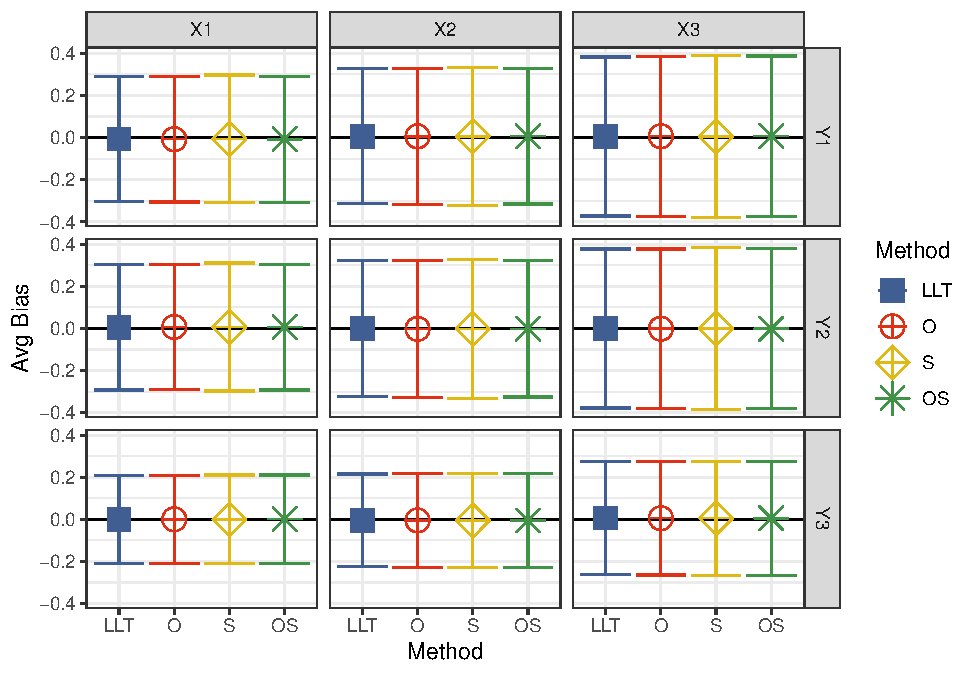
\includegraphics{Master_files/figure-latex/unnamed-chunk-22-1.pdf}
\caption{\label{fig:unnamed-chunk-22}Bias and Estimate Variability}
\end{figure}

\textbackslash begin\{table\}

\textbackslash caption\{\label{tab:unnamed-chunk-23}Covariance estimate (coverage \%)\}
\centering

\begin{tabular}[t]{ccccccc}
\toprule
 & Parameter & True value & LLT & O & S & OS\\
\midrule
\addlinespace[0.3em]
\multicolumn{7}{l}{\textbf{Observation Error}}\\
\hspace{1em} & 1,1 & 15 & 14.909 (95\%) & 14.919 (95.1\%) & 14.688 (92.8\%) & 14.95 (94.8\%)\\
\cmidrule{2-7}
\hspace{1em} & 1,2 & 2.4 & - & 2.371 (95.3\%) & - & 2.425 (94.1\%)\\
\cmidrule{2-7}
\hspace{1em} & 2,2 & 15 & 14.892 (94.4\%) & 14.903 (94.9\%) & 14.668 (93.4\%) & 14.927 (94.6\%)\\
\cmidrule{2-7}
\hspace{1em} & 1,3 & 1 & - & 0.99 (95.6\%) & - & 1.027 (95.6\%)\\
\cmidrule{2-7}
\hspace{1em} & 2,3 & 1 & - & 0.988 (95.2\%) & - & 1.008 (94.7\%)\\
\cmidrule{2-7}
\hspace{1em} & 3,3 & 10 & 10.056 (95.1\%) & 10.063 (94.5\%) & 10.021 (94.7\%) & 10.093 (95.1\%)\\
\cmidrule{1-7}
\addlinespace[0.3em]
\multicolumn{7}{l}{\textbf{State Process}}\\
\hspace{1em} & 1,1 & 5 & 4.89 (93.5\%) & 4.969 (94.8\%) & 5.206 (93.8\%) & 4.985 (94.5\%)\\
\cmidrule{2-7}
\hspace{1em} & 1,2 & 0 & - & - & 0.987 (50\%) & -0.071 (93.9\%)\\
\cmidrule{2-7}
\hspace{1em} & 2,2 & 5 & 4.887 (94.8\%) & 4.964 (95.2\%) & 5.205 (95.5\%) & 4.988 (95.1\%)\\
\cmidrule{2-7}
\hspace{1em} & 1,3 & 0 & - & - & 0.373 (81.5\%) & -0.042 (94.2\%)\\
\cmidrule{2-7}
\hspace{1em} & 2,3 & 0 & - & - & 0.386 (78.3\%) & -0.021 (93.3\%)\\
\cmidrule{2-7}
\hspace{1em} & 3,3 & 2 & 1.893 (92\%) & 1.932 (93.6\%) & 1.973 (93\%) & 1.932 (93.4\%)\\
\bottomrule
\end{tabular}

\textbackslash end\{table\}

\raggedright

\hypertarget{s-model-1}{%
\subsubsection{S Model}\label{s-model-1}}

\begin{table}

\caption{\label{tab:unnamed-chunk-25}Linear effect coverage percentage.}
\centering
\begin{tabular}[t]{llrllll}
\toprule
Test & Variable & Beta & LLT & O & S & OS\\
\midrule
Y1 & X1 & 4 & 95.4\% & 95.6\% & 95.7\% & 95.9\%\\
Y1 & X2 & 2 & 94.6\% & 95.1\% & 95\% & 95.6\%\\
Y1 & X3 & 1 & 95.9\% & 95.7\% & 95.8\% & 95.7\%\\
Y2 & X1 & -3 & 95.7\% & 96.5\% & 95.5\% & 96.1\%\\
Y2 & X2 & 0 & 94.1\% & 94.3\% & 94.8\% & 95.1\%\\
\addlinespace
Y2 & X3 & 1 & 95.3\% & 95.7\% & 95.5\% & 95.7\%\\
Y3 & X1 & 0 & 94.5\% & 94.8\% & 94.6\% & 94.5\%\\
Y3 & X2 & 0 & 95\% & 95.4\% & 94.9\% & 95.8\%\\
Y3 & X3 & 0 & 93.8\% & 94.2\% & 93.9\% & 93.8\%\\
\bottomrule
\end{tabular}
\end{table}

\begin{figure}
\centering
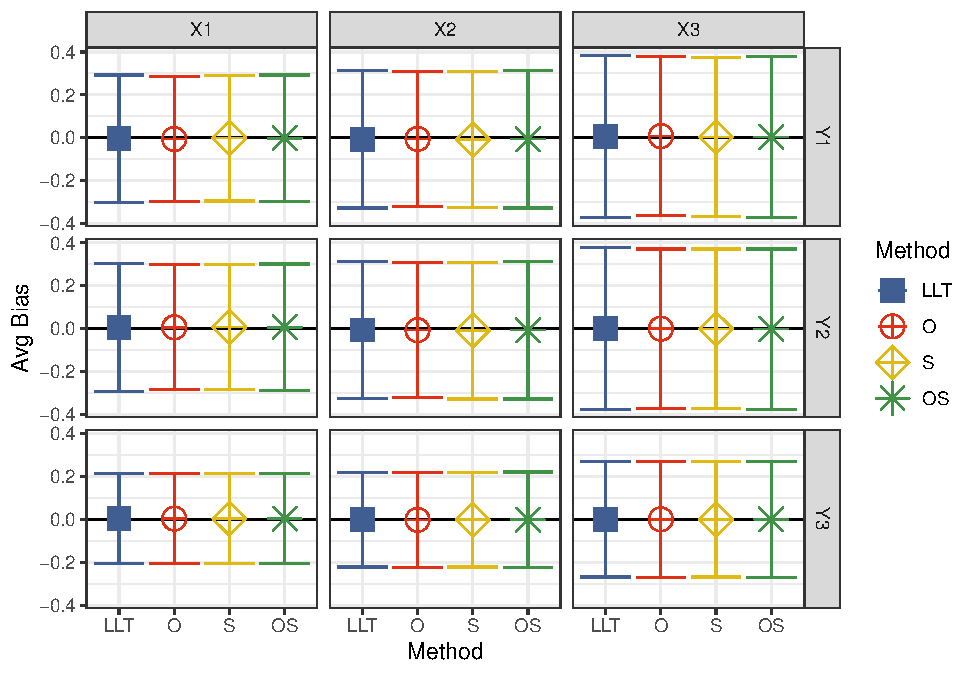
\includegraphics{Master_files/figure-latex/unnamed-chunk-26-1.pdf}
\caption{\label{fig:unnamed-chunk-26}Bias and Estimate Variability}
\end{figure}

\textbackslash begin\{table\}

\textbackslash caption\{\label{tab:unnamed-chunk-27}Covariance estimate (coverage \%)\}
\centering

\begin{tabular}[t]{ccccccc}
\toprule
 & Parameter & True value & LLT & O & S & OS\\
\midrule
\addlinespace[0.3em]
\multicolumn{7}{l}{\textbf{Observation Error}}\\
\hspace{1em} & 1,1 & 15 & 14.866 (94.9\%) & 15.248 (94.9\%) & 15.147 (93.8\%) & 15.065 (93.5\%)\\
\cmidrule{2-7}
\hspace{1em} & 1,2 & 0 & - & 2.436 (2.9\%) & - & -0.387 (90.4\%)\\
\cmidrule{2-7}
\hspace{1em} & 2,2 & 15 & 14.908 (95\%) & 15.293 (93.5\%) & 15.18 (93.6\%) & 15.092 (93.5\%)\\
\cmidrule{2-7}
\hspace{1em} & 1,3 & 0 & - & 0.012 (95.9\%) & - & 0.006 (95.5\%)\\
\cmidrule{2-7}
\hspace{1em} & 2,3 & 0 & - & -0.02 (95.2\%) & - & -0.033 (94.6\%)\\
\cmidrule{2-7}
\hspace{1em} & 3,3 & 10 & 10.06 (94.5\%) & 10.064 (94.8\%) & 10.087 (94.8\%) & 10.102 (94.7\%)\\
\cmidrule{1-7}
\addlinespace[0.3em]
\multicolumn{7}{l}{\textbf{State Process}}\\
\hspace{1em} & 1,1 & 5 & 4.879 (93.2\%) & 4.59 (90.8\%) & 4.803 (92.2\%) & 4.94 (93\%)\\
\cmidrule{2-7}
\hspace{1em} & 1,2 & 3.714 & - & - & 3.786 (94.6\%) & 3.98 (91.8\%)\\
\cmidrule{2-7}
\hspace{1em} & 2,2 & 5 & 4.899 (93.7\%) & 4.606 (90.2\%) & 4.838 (91.3\%) & 4.977 (91.1\%)\\
\cmidrule{2-7}
\hspace{1em} & 1,3 & 0 & - & - & 0.017 (95.1\%) & 0.015 (93.5\%)\\
\cmidrule{2-7}
\hspace{1em} & 2,3 & 0 & - & - & 0.003 (95\%) & 0.015 (93.3\%)\\
\cmidrule{2-7}
\hspace{1em} & 3,3 & 2 & 1.89 (92.7\%) & 1.932 (93.7\%) & 1.916 (92.2\%) & 1.928 (92.7\%)\\
\bottomrule
\end{tabular}

\textbackslash end\{table\}

\raggedright

\hypertarget{os-model-1}{%
\subsubsection{OS Model}\label{os-model-1}}

\begin{table}

\caption{\label{tab:unnamed-chunk-29}Linear effect coverage percentage.}
\centering
\begin{tabular}[t]{llrllll}
\toprule
Test & Variable & Beta & LLT & O & S & OS\\
\midrule
Y1 & X1 & 4 & 96.2\% & 94.8\% & 96.8\% & 96.1\%\\
Y1 & X2 & 2 & 94.6\% & 93.4\% & 95.5\% & 94.5\%\\
Y1 & X3 & 1 & 95.2\% & 94.1\% & 95.8\% & 95\%\\
Y2 & X1 & -3 & 95\% & 94.4\% & 95.8\% & 95.7\%\\
Y2 & X2 & 0 & 94.5\% & 93.1\% & 95.9\% & 95.2\%\\
\addlinespace
Y2 & X3 & 1 & 94.9\% & 94\% & 96.8\% & 96.4\%\\
Y3 & X1 & 0 & 95.7\% & 96.2\% & 96\% & 95.7\%\\
Y3 & X2 & 0 & 95\% & 94.7\% & 94.9\% & 95.2\%\\
Y3 & X3 & 0 & 94.5\% & 94.8\% & 94.9\% & 94.9\%\\
\bottomrule
\end{tabular}
\end{table}

\begin{figure}
\centering
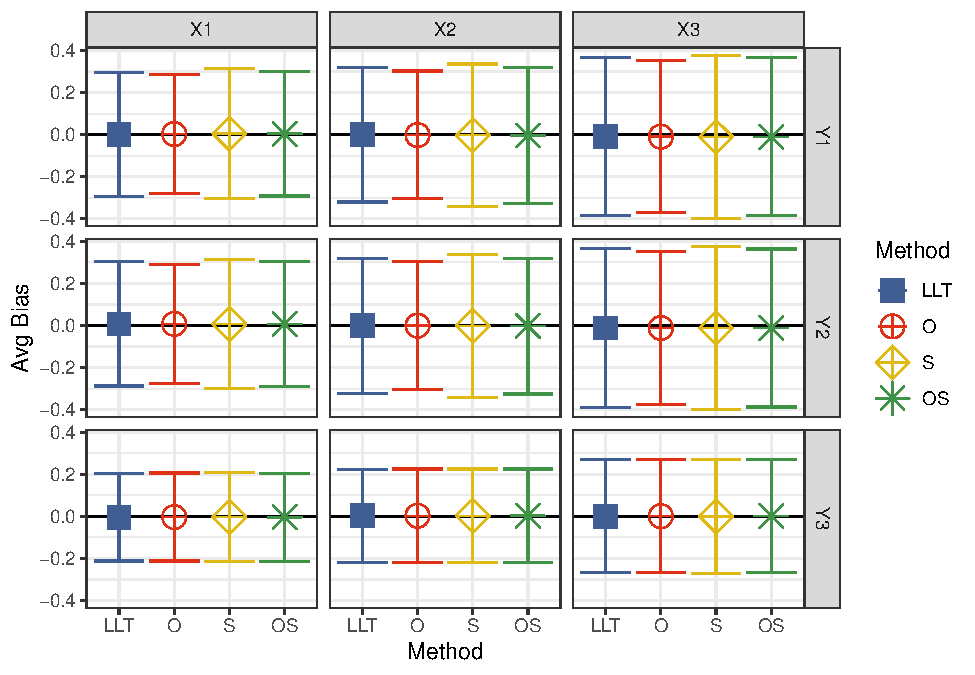
\includegraphics{Master_files/figure-latex/unnamed-chunk-30-1.pdf}
\caption{\label{fig:unnamed-chunk-30}Bias and Estimate Variability}
\end{figure}

\textbackslash begin\{table\}

\textbackslash caption\{\label{tab:unnamed-chunk-31}Covariance estimate (coverage \%)\}
\centering

\begin{tabular}[t]{ccccccc}
\toprule
 & Parameter & True value & LLT & O & S & OS\\
\midrule
\addlinespace[0.3em]
\multicolumn{7}{l}{\textbf{Observation Error}}\\
\hspace{1em} & 1,1 & 15 & 14.964 (94.4\%) & 15.752 (88.2\%) & 14.273 (86.7\%) & 15.075 (94.3\%)\\
\cmidrule{2-7}
\hspace{1em} & 1,2 & 2.4 & - & 4.976 (2.4\%) & - & 2.14 (91.7\%)\\
\cmidrule{2-7}
\hspace{1em} & 2,2 & 15 & 14.948 (94.1\%) & 15.733 (87.9\%) & 14.248 (85.1\%) & 15.066 (93.8\%)\\
\cmidrule{2-7}
\hspace{1em} & 1,3 & 1 & - & 0.997 (94.6\%) & - & 0.979 (94.2\%)\\
\cmidrule{2-7}
\hspace{1em} & 2,3 & 1 & - & 1.008 (94.8\%) & - & 0.997 (92.6\%)\\
\cmidrule{2-7}
\hspace{1em} & 3,3 & 10 & 10.021 (93.7\%) & 10.021 (93.5\%) & 9.988 (93.7\%) & 10.056 (93.1\%)\\
\cmidrule{1-7}
\addlinespace[0.3em]
\multicolumn{7}{l}{\textbf{State Process}}\\
\hspace{1em} & 1,1 & 5 & 4.835 (94\%) & 4.168 (78\%) & 5.776 (82.8\%) & 4.941 (94.2\%)\\
\cmidrule{2-7}
\hspace{1em} & 1,2 & 3.714 & - & - & 5.007 (44.7\%) & 3.891 (93.7\%)\\
\cmidrule{2-7}
\hspace{1em} & 2,2 & 5 & 4.849 (92.4\%) & 4.183 (78.9\%) & 5.8 (82\%) & 4.952 (92.7\%)\\
\cmidrule{2-7}
\hspace{1em} & 1,3 & 0 & - & - & 0.47 (71.9\%) & -0.009 (93.8\%)\\
\cmidrule{2-7}
\hspace{1em} & 2,3 & 0 & - & - & 0.47 (73.8\%) & -0.015 (93.9\%)\\
\cmidrule{2-7}
\hspace{1em} & 3,3 & 2 & 1.894 (92.6\%) & 1.943 (93.8\%) & 1.977 (93\%) & 1.939 (93\%)\\
\bottomrule
\end{tabular}

\textbackslash end\{table\}

\raggedright

\hypertarget{real-data-simulation}{%
\subsection{Real Data Simulation}\label{real-data-simulation}}

To test the validity of the MLLT model on real cognition data, a real data simulation is conducted on the unmatched that transitioned to dementia during follow up (section \ref{DAT}). For this simulation, participants are randomized to one of two groups. One of the randomized groups having no change to their outcomes and the other group receiving an added constant linear effect to each of the NACC outcomes. Although we do not know the true data generation process or the inter-relation between each test, we do know the true simulated ``group'' effect. The primary aim of the MLLT as presented is not specifically for modeling linear effects, but by estimating linear effects we are able to assess overall model validity. To declare model adequacy we desire a model that has low bias, low parameter variance (assessed by small confidence intervals), and proper 95\% parameter coverage.

Using a similar simulation strategy, the LLT was established to model the NACC battery data well {[}{]} and, for this reason, the LLT was used as a baseline comparison. The LLT is fit to each outcome while controlling for the covariates of interest (section \ref{MOI}) as well as the simulated group effect. Three separate MLLT models are fit to the data that each carry different modeling assumptions: 1.) correlation only exists in the observation equation (O), 2.) correlation only exists in the state equation (S), and 3.) correlation exists in both the observation and state equation (OS). For each of the models, 5000 iterations of the Gibb's sampler is carried out with a burn-in of 2000. The process of randomizing each participant to a group with, one having an added linear effect, and estimating the group effect with each model is repeated 1,000 times. The group effect was chosen to be 1 for each outcome.

\hypertarget{real-data-simulation-results}{%
\subsubsection{Real Data Simulation Results}\label{real-data-simulation-results}}

When estimating the randomized group effects the LLT, O, S, and OS models all maintain unbiasedness. The LLT, S, and OS are all able to maintain near 95\% coverage of the true linear effect. However, the O model tends to undercover the true parameter as seen in table {[}{]} (average coverage of 0.90), indicating that this model does not fit the model as well. The confidence interval for the O model is tightest, which would indicate higher power, but because the O model doesn't maintain 95\% coverage the result is inconsequential. The S and OS models maintain the desired confidence interval lengths when compared to the baseline independent models.

Reasoning for the ill-fitting model O can be observed in the estimated observation and state correlation matrices in the OS model {[}figure\_, figure\_{]}. When estimating both correlation matrices, very little correlation is placed in the observation equation, except for moderate correlation between MEMUNITS and LOGIMEM (cor = 0.47). The next highest correlation is between the ANIMALS and VEG naming (cor = 0.13). However, there is very high correlation placed in the state equation matrix with the lowest correlation being between TRAILA and MEMUNITS (cor = 0.30) and the highest correlation between MEMUNITS and LOGIMEM (cor = 0.97). These findings emphasize the importance of the underlying cognitive state process and the inter-relation of this processes between cognitive tests. When the underlying state correlation goes unaccounted for, it leads to too much correlation going into the observation equation in the O model and faulty estimates.

If the primary concern of analysis is to estimate the underlying state process correlation, both the S and OS models can be seen as valid. For the NACC data, if power is of concern, one may decide to use the S model as there are 45 fewer covariance parameters to estimate and there is generally very low correlation in the observation equation. In our analysis, eliminating the covariance in the observation does not seem to increase power a significant amount and by eliminating the observation covariance could add bias to the state covariance estimate.

\begin{table}

\caption{\label{tab:unnamed-chunk-33}Linear effect coverage.}
\centering
\begin{tabular}[t]{lllll}
\toprule
  & LLT & O & S & OS\\
\midrule
ANIMALS & 94.1\% & 90.9\% & 93.9\% & 94.9\%\\
BOSTON & 93.5\% & 91.8\% & 92.1\% & 92.9\%\\
DIGIB & 94.1\% & 92.9\% & 93.9\% & 94.1\%\\
DIGIF & 94.3\% & 93.8\% & 95.5\% & 94.2\%\\
LOGIMEM & 96.1\% & 86.2\% & 97.1\% & 97\%\\
\addlinespace
MEMUNITS & 96.5\% & 87.7\% & 97.9\% & 96.6\%\\
TRAILA & 93.9\% & 89.8\% & 93.8\% & 92.9\%\\
TRAILB & 95.2\% & 88.6\% & 93.2\% & 94.4\%\\
WAIS & 94.9\% & 90.3\% & 94.2\% & 95.1\%\\
\bottomrule
\end{tabular}
\end{table}

\begin{figure}
\centering
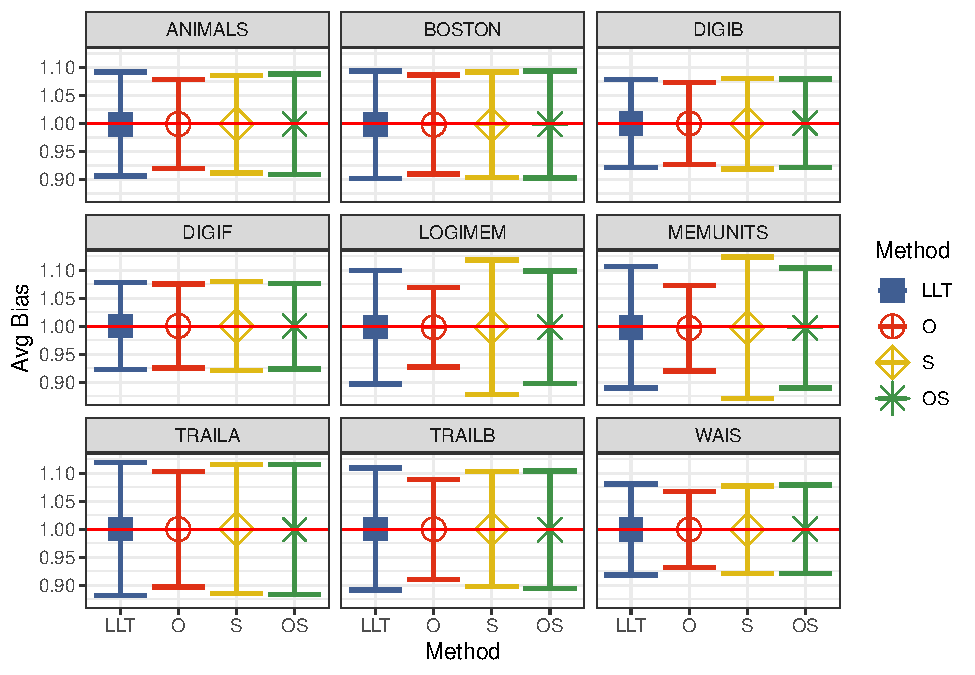
\includegraphics{Master_files/figure-latex/unnamed-chunk-34-1.pdf}
\caption{\label{fig:unnamed-chunk-34}Linear effect bias and estimate variability.}
\end{figure}

\begin{figure}
\centering
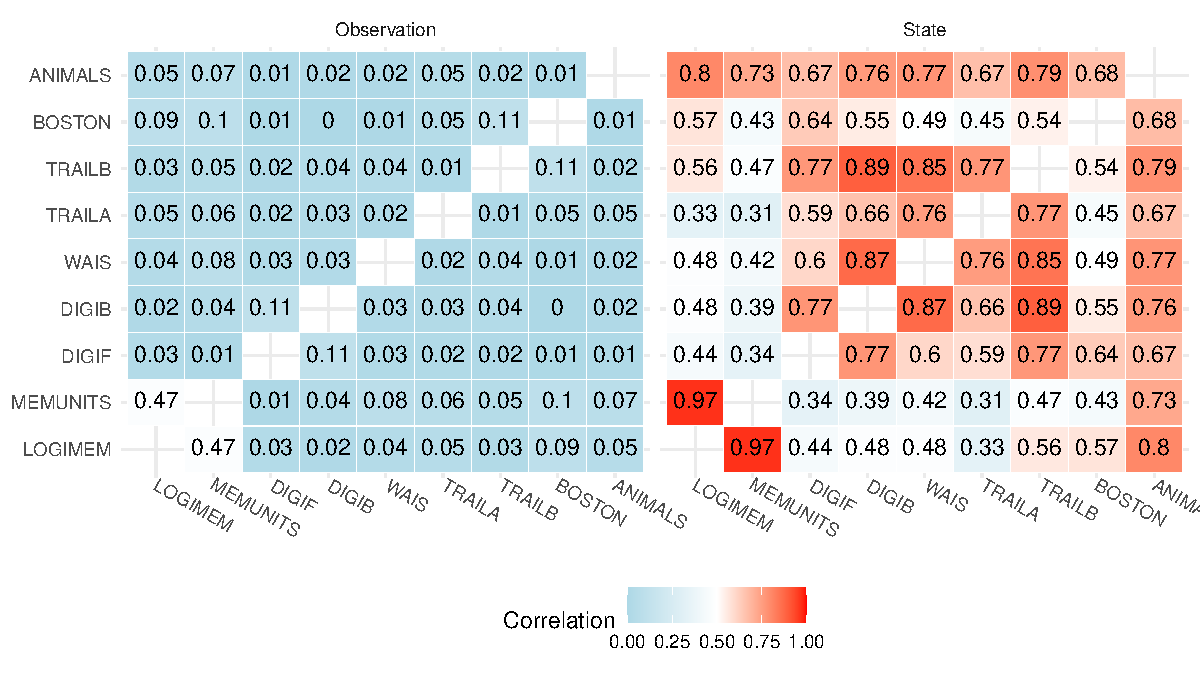
\includegraphics{Master_files/figure-latex/unnamed-chunk-35-1.pdf}
\caption{\label{fig:unnamed-chunk-35}OS model observation error and state process correlation estimates.}
\end{figure}

\hypertarget{data-analysis}{%
\section{Data Analysis}\label{data-analysis}}

To compare latent process correlation between those who transitioned to MCI or dementia during follow-up and those who did not, we fit the MLLT model which allows correlation in the observation errors and underlying cognitive process (OS) using the model of interest described in section \ref{MOI}. The model is fit on the full data and sensitivity analysis matched data described in section \ref{DAT}. The Gibb's sampling was repeated 5,000 times with a burn-in of 2,000 samples, resulting in 3,000 samples for parameter inference. Non-informative priors are used for both the linear effects and covariance matrices.

\hypertarget{data-analysis-results}{%
\subsection{Data Analysis Results}\label{data-analysis-results}}

In both the dementia and non-dementia groups, there is very little estimated observation correlation. Instead, the correlation is primarily placed in the state equation. In the non-dementia population, there are much distinct correlation clusters in memory (LOGIMEM, MEMUNITS), digit (DIGIB, DIGIF), and executive function (TRAILA, TRAILB, WAIS) in the estimated state correlation process. The dementia population generally has much higher correlation in the state equation. The digit and executive function blocks share much higher cross correlation than the non-dementia group. The Animals test generally has low correlation for the non-dementia population and very high correlation with all other tests in the population that transitioned to MCI or dementia.

As expected by the correlation estimates, 23 of the 36 correlation coefficients share less than 5\% overlap in posterior draw distributions.

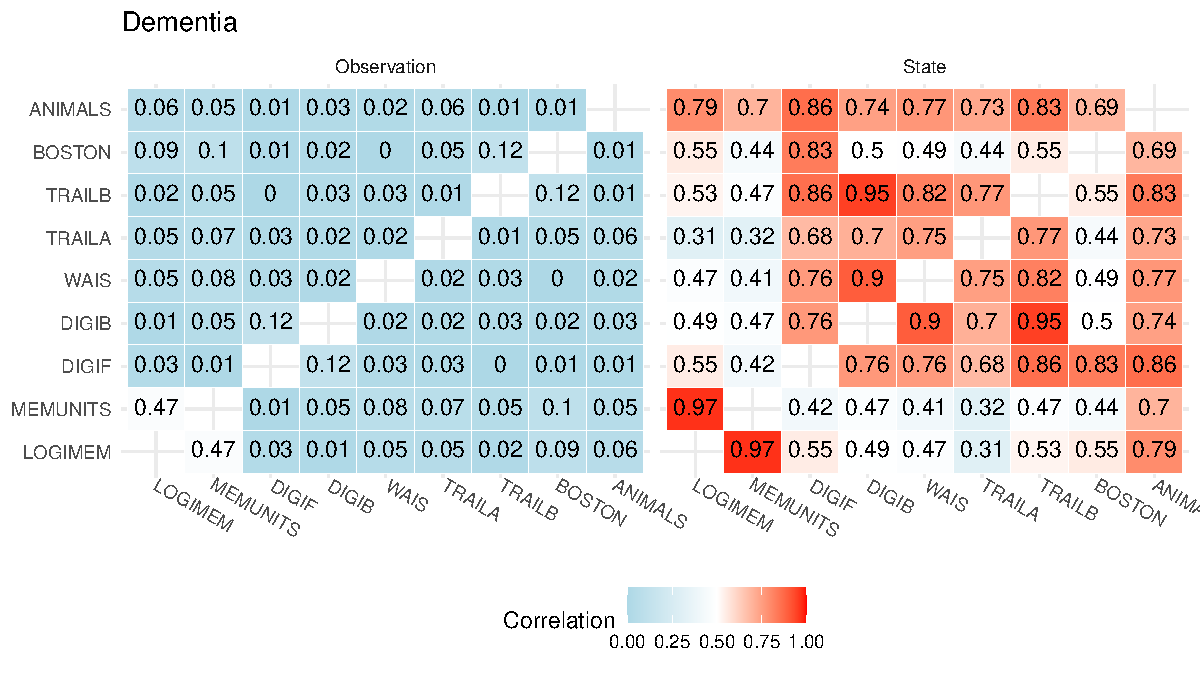
\includegraphics{Master_files/figure-latex/unnamed-chunk-38-1.pdf}

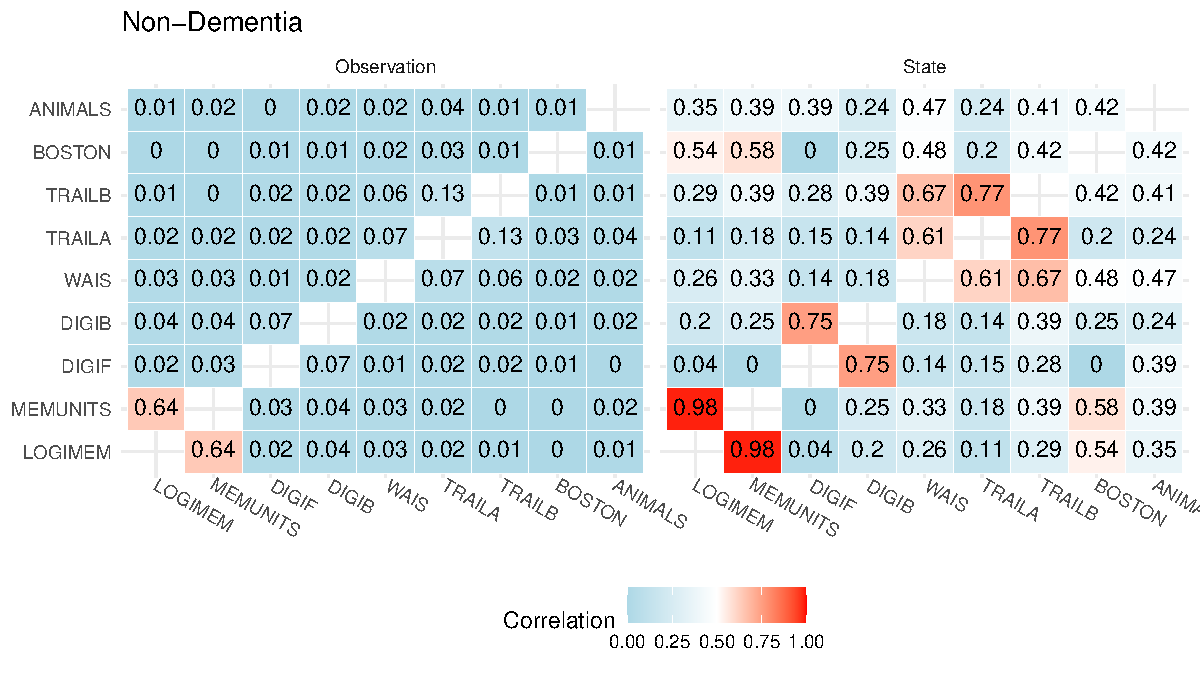
\includegraphics{Master_files/figure-latex/unnamed-chunk-40-1.pdf}

\hypertarget{state-correlation-posterior-differences}{%
\subsubsection{State Correlation Posterior Differences}\label{state-correlation-posterior-differences}}

h

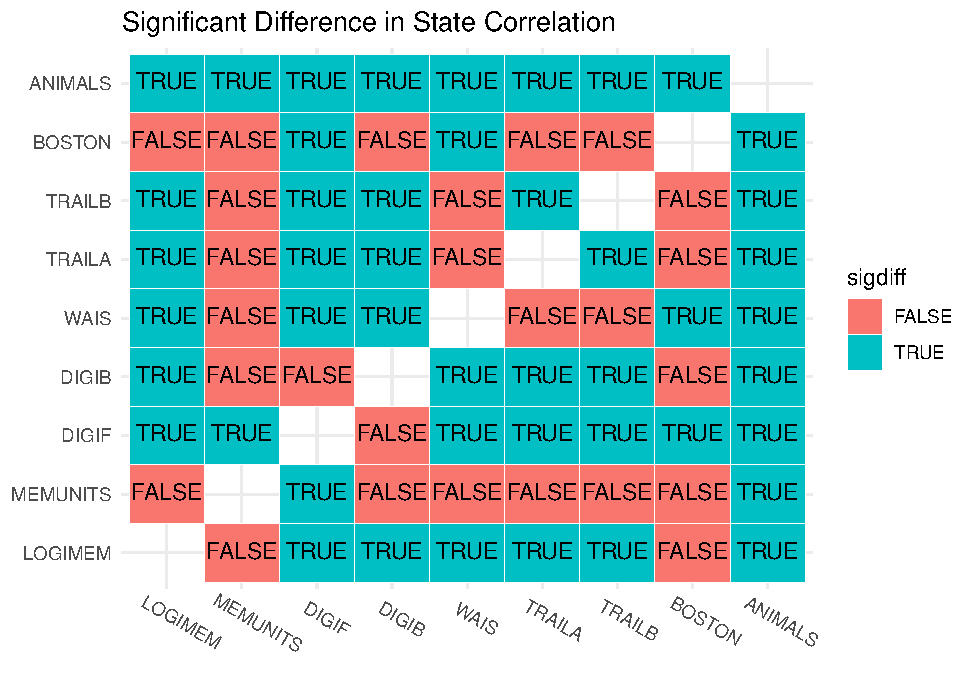
\includegraphics{Master_files/figure-latex/unnamed-chunk-42-1.pdf}

\begin{itemize}
\tightlist
\item
  \textbf{BLUE} is \textbf{Non-Dementia}
\item
  \textbf{RED} is \textbf{Dementia}
\end{itemize}

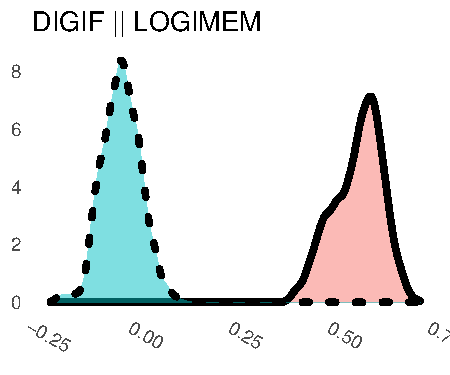
\includegraphics{Master_files/figure-latex/unnamed-chunk-43-1.pdf} 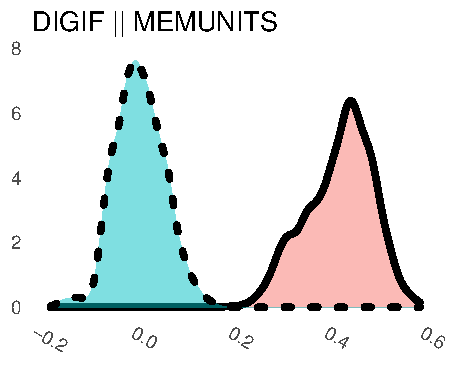
\includegraphics{Master_files/figure-latex/unnamed-chunk-43-2.pdf} 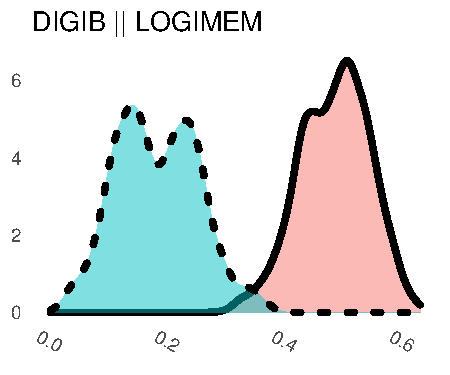
\includegraphics{Master_files/figure-latex/unnamed-chunk-43-3.pdf} 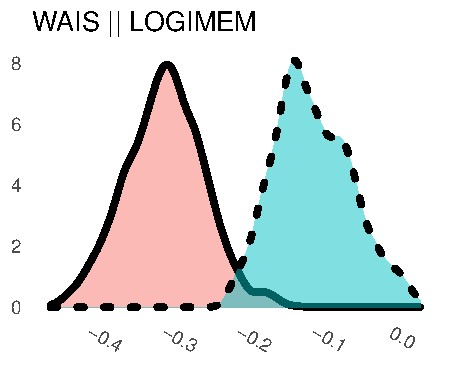
\includegraphics{Master_files/figure-latex/unnamed-chunk-43-4.pdf} 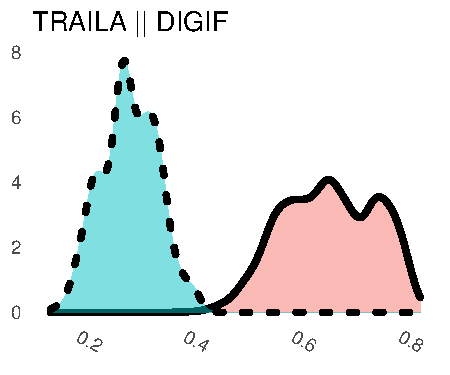
\includegraphics{Master_files/figure-latex/unnamed-chunk-43-5.pdf} 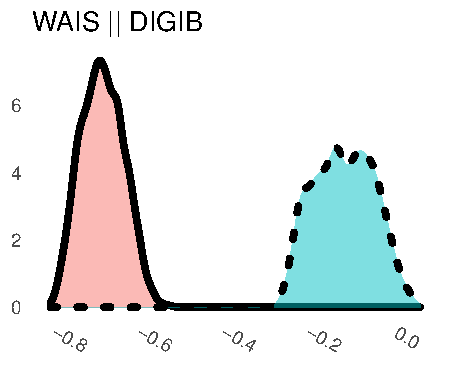
\includegraphics{Master_files/figure-latex/unnamed-chunk-43-6.pdf} 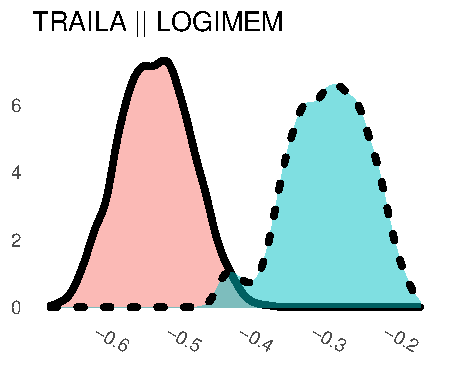
\includegraphics{Master_files/figure-latex/unnamed-chunk-43-7.pdf} 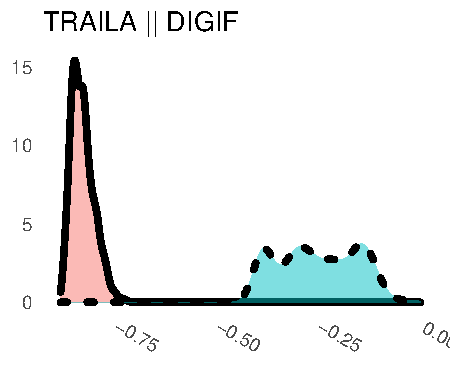
\includegraphics{Master_files/figure-latex/unnamed-chunk-43-8.pdf} 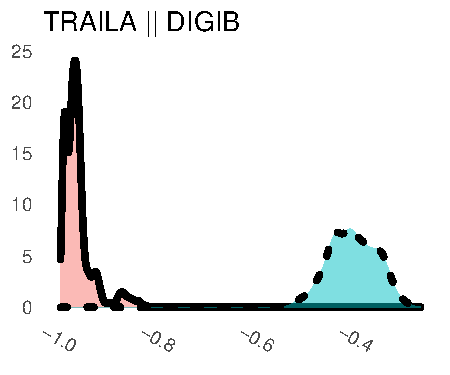
\includegraphics{Master_files/figure-latex/unnamed-chunk-43-9.pdf} 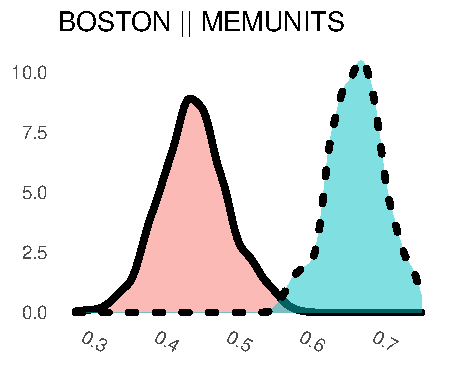
\includegraphics{Master_files/figure-latex/unnamed-chunk-43-10.pdf} 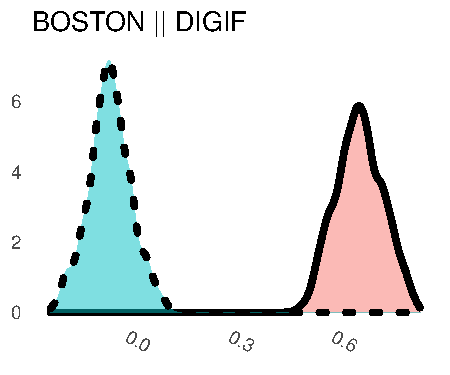
\includegraphics{Master_files/figure-latex/unnamed-chunk-43-11.pdf} 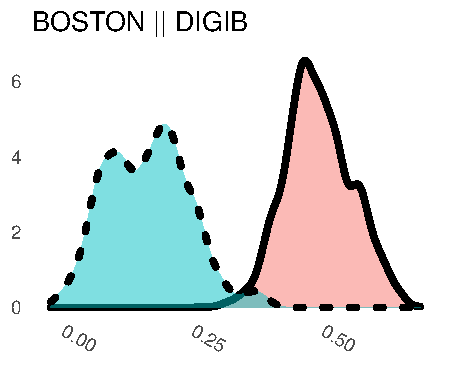
\includegraphics{Master_files/figure-latex/unnamed-chunk-43-12.pdf} 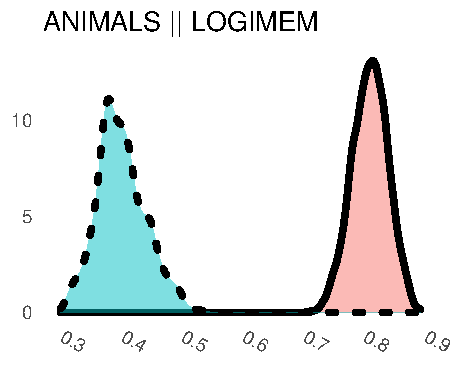
\includegraphics{Master_files/figure-latex/unnamed-chunk-43-13.pdf} 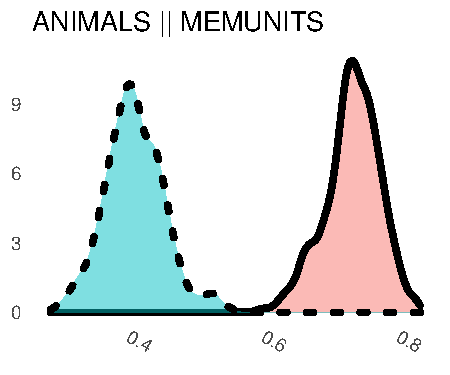
\includegraphics{Master_files/figure-latex/unnamed-chunk-43-14.pdf} 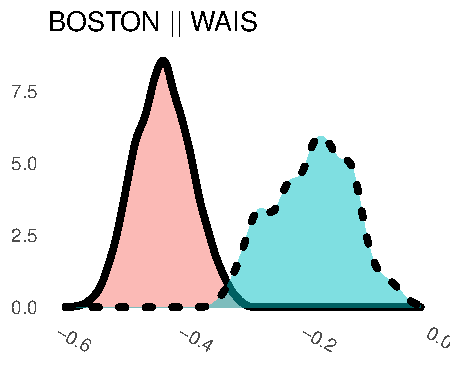
\includegraphics{Master_files/figure-latex/unnamed-chunk-43-15.pdf} 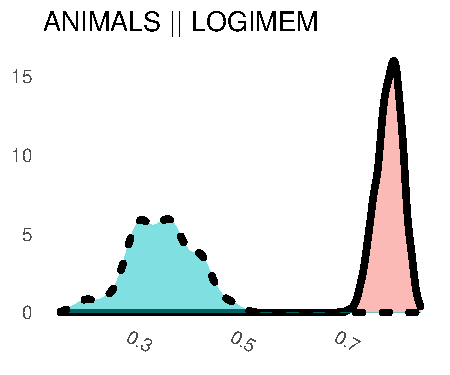
\includegraphics{Master_files/figure-latex/unnamed-chunk-43-16.pdf} 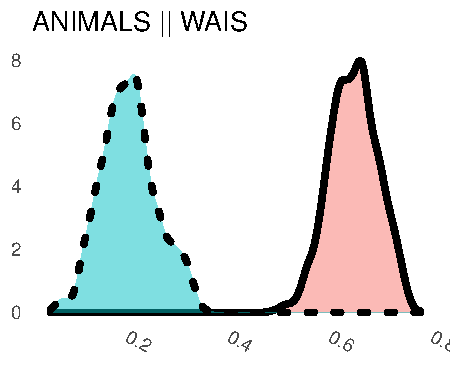
\includegraphics{Master_files/figure-latex/unnamed-chunk-43-17.pdf} 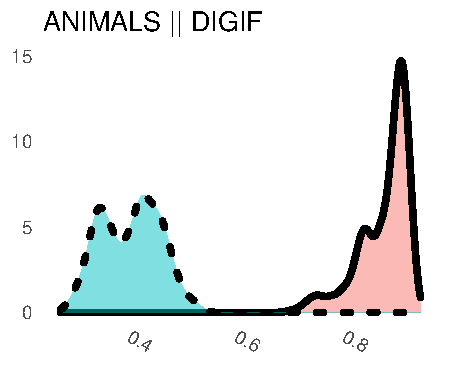
\includegraphics{Master_files/figure-latex/unnamed-chunk-43-18.pdf} 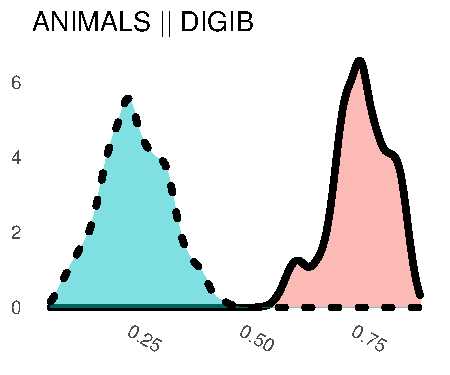
\includegraphics{Master_files/figure-latex/unnamed-chunk-43-19.pdf} 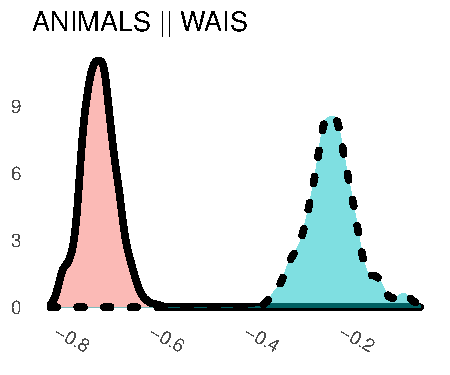
\includegraphics{Master_files/figure-latex/unnamed-chunk-43-20.pdf}

\hypertarget{sensitivity}{%
\subsubsection{Sensitivity}\label{sensitivity}}

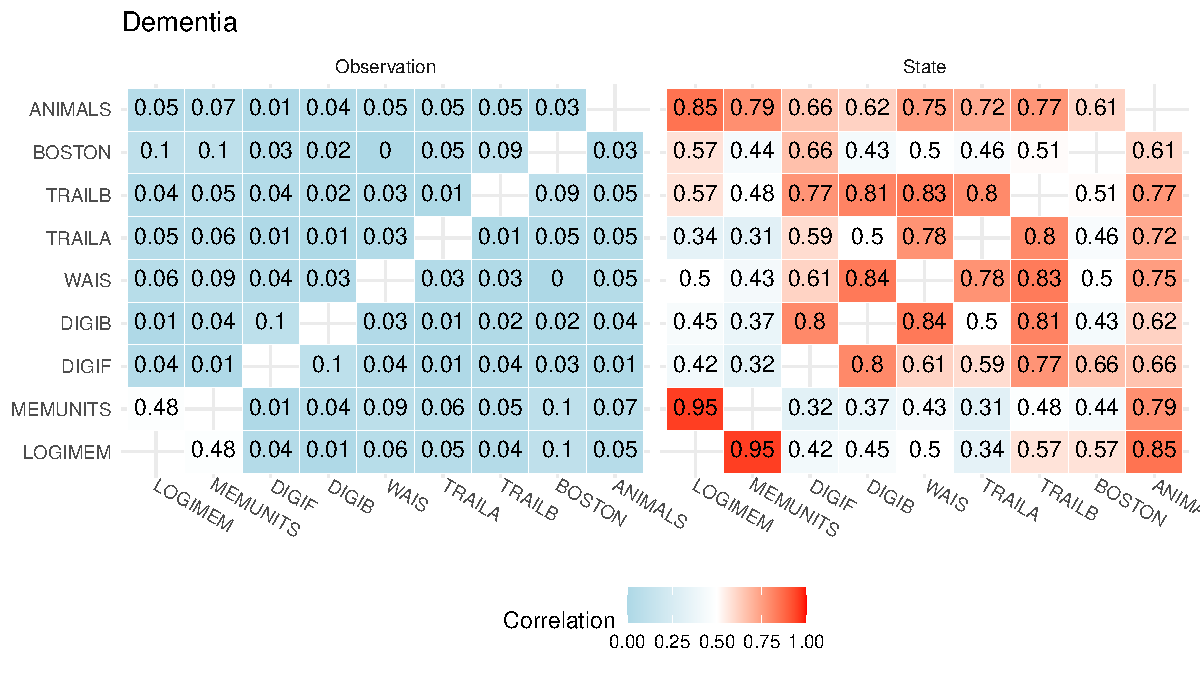
\includegraphics{Master_files/figure-latex/unnamed-chunk-44-1.pdf}

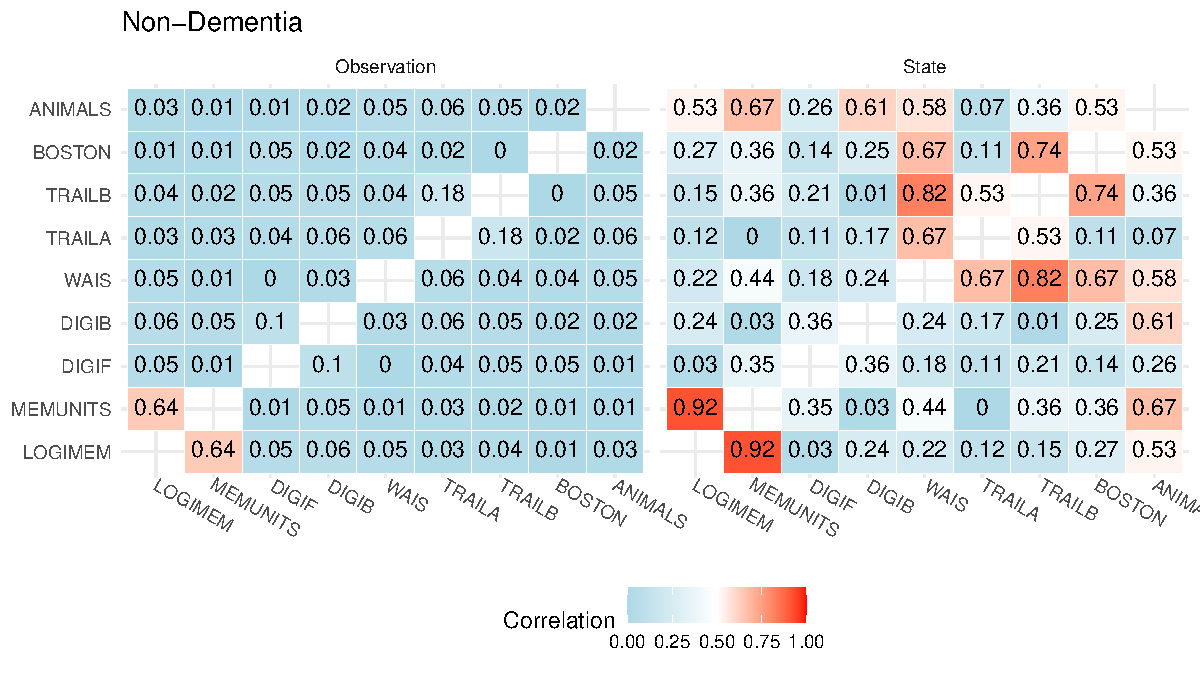
\includegraphics{Master_files/figure-latex/unnamed-chunk-45-1.pdf}

\hypertarget{discussion}{%
\section{Discussion}\label{discussion}}

The multivariate local linear trend state space model was developed to assess inter-relationships between cognitive tests spanning different cognition domains. It achieves this by modeling the correlation between tests in both the observation equation and the underlying cognition process equation, after accounting for linear effects. By controlling for linear effects we are able to control for possible cohort difference when estimating the inter-relatedness.

The fully simulated data simulation shows the MLLT where, correlation is assumed in the observation and state equations, is the most robust model for the varying correlation assumptions. This MLLT was able to accurately estimate the inter-relatedness of the simulated cognitive tests in both the observation and state equations. In addition, the MLLT also as proficient as the LLT in estimating linear effects on the outcome.

The real data simulation provided insight into how the MLLT performs on real data provided by the NACC. The OS and S MLLT models were able to accurately estimate the added linear effect on the real outcomes and were as accurate as the proven LLT model. The O MLLT suffered in terms of proper 95\% confidence interval coverage. Reasoning was made apparent by the correlation structure estimated by the OS model, which put very low covariance in the observation equation and high covariance in the state equation. These results help confirm the true underlying data generation process is more likely that of an S or OS model. The findings also support the importance in estimating the underlying cognition process unaccounted for by the linear effects of interest.

Similar to the LLT, the dynamic MLLT is able to estimate linear effects of interest well, but, unlike the LLT, the MLLT can also provide accurate inference of linear effects across different cognitive outcomes. To test if an independent variable has a significantly different effect between tests, we rely on outcome standardization, which relies on accurate estimation of the observation error correlation matrix. Pre-standardizing the data is ineffective as, according to our model, variation in the outcome can come from the measurement error or from the latent cognition process. For this reason we propose standardizing the outcome during each step of the Bayesian Gibb's sampler.

Depending on statistical power and the objectives of an analysis, different assumptions of the underlying model can be assumed. First, it can be assumed that correlation in the observations exists only in the observation errors. This assumption can be made when linear effects and cross test linear effect comparisons are of primary interest. Next, it can be assumed that the correlation exists only in the underlying latent cognition process. This can be used when the primary focus of the analysis is understanding latent constructs of cognition. However, for an ample sample size we can assume that there is correlation in the observation error and in the latent cognition process. This is the proffered model and provides the most accurate results regardless of analysis aims.

\newpage{}

\hypertarget{bibliography}{%
\section*{Bibliography}\label{bibliography}}
\addcontentsline{toc}{section}{Bibliography}

\hypertarget{refs}{}
\begin{CSLReferences}{1}{0}
\leavevmode\vadjust pre{\hypertarget{ref-Alz_assoc}{}}%
{``2022 Alzheimer's Disease Facts and Figures.''} 2022. \emph{Alzheimers Dement}. Alzheimer's Association. \url{https://www.alz.org/media/documents/alzheimers-facts-and-figures.pdf}.

\leavevmode\vadjust pre{\hypertarget{ref-ChapmanRobertM2010DoAd}{}}%
Chapman, Robert M, Mark Mapstone, Anton P Porsteinsson, Margaret N Gardner, John W McCrary, Elizabeth DeGrush, Lindsey A Reilly, Tiffany C Sandoval, and Maria D Guillily. 2010. {``Diagnosis of Alzheimer's Disease Using Neuropsychological Testing Improved by Multivariate Analyses.''} \emph{Journal of Clinical and Experimental Neuropsychology} 32 (8): 793--808.

\leavevmode\vadjust pre{\hypertarget{ref-HAYDENKathleenM2011FSot}{}}%
HAYDEN, Kathleen M, Richard N JONES, Catherine ZIMMER, Brenda L PLASSMAN, Jeffrey N BROWNDYKE, Carl PIEPER, Lauren H WARREN, and Kathleen A WELSH-BOHMER. 2011. {``Factor Structure of the National Alzheimer's Coordinating Centers Uniform Dataset Neuropsychological Battery: An Evaluation of Invariance Between and Within Groups over Time.''} \emph{Alzheimer Disease and Associated Disorders} 25 (2): 128--37.

\end{CSLReferences}

\end{document}
